%=========================================================================%
%   LaTeX File for Master thesis of Sun Yat-Sen University
%-------------------------------------------------------------------------%
%   Copyright 2004  by      (FBI@BHQT)
%-------------------------------------------------------------------------%
%   Latex 硕士论文模板
%   在ctex2.3.3(miktex2.3)、ctex2.4.6完全安装下通过测试.
%   本模板使用ctex.org的cjk版本
%   -- 经刘成明根据大连理工大学研究生院2007-6-5发布的博士学位论文模板修改而成。
%      2008年5月8日根据中山大学研究生院最新模板修订。
%   -- 2009年4月经车春回根据刘成明老师的博士论文模板修改而成,符合中山大学硕士
%      硕士研究生要求。
%=========================================================================%

\documentclass[12pt,openany,a4paper,twoside]{book}
%algorithm和algorithmic这两个宏包用于画伪代码
\usepackage{algorithm}
\usepackage{algpseudocode}
%使用booktab宏包定义三条划线命令:\toprule、\midrule 和 \bottomrule
%用于画三线表
\usepackage{booktabs}
\usepackage{amsmath,amssymb}



\renewcommand{\algorithmicrequire}{ \textbf{Input:}} %Use Input in the format of Algorithm
\renewcommand{\algorithmicensure}{ \textbf{Output:}} %UseOutput in the format of Algorithm
\newcommand{\algrule}[1][.2pt]{\par\vskip.5\baselineskip\hrule height #1\par\vskip.5\baselineskip}

%=========================================================================%
%                          引用的宏包和相应的定义
%\usepackage{overcite}
%\usepackage[super]{natbib}
%=========================================================================%

%============================ 中文支持宏包 ==============================%
\usepackage[BoldFont,SlantFont]{xeCJK}
\usepackage{CJKnumb}
%====================== 图形和超链接支持宏包 ========================%
\usepackage[CJKbookmarks=true,
            bookmarksnumbered=true,
            bookmarksopen=true,
            colorlinks=true, %注释掉此项则交叉引用为彩色边框(将colorlinks和pdfborder同时注释掉)
            pdfborder=001,   %注释掉此项则交叉引用为彩色边框
            citecolor=blue,%
            linkcolor=blue
            ]{hyperref}

\usepackage{booktabs}
\usepackage{amsmath,amssymb}

\usepackage[numbers,sort&compress]{natbib}
\usepackage{color}              % 支持彩色
\usepackage{subfigure}          % 支持子图
\usepackage{floatflt}           % 图文混排用宏包
\usepackage{rotating}           % 图形和表格的控制
\usepackage{flafter}            % 因为图形可浮动到当前页的顶部,所以它可能会出现
                                % 在它所在文本的前面. 要防止这种情况,可使用 flafter
                                % 宏包
\usepackage[below]{placeins}    %浮动图形控制宏包
                                %允许上一个section的浮动图形出现在下一个
                                %section的开始部分该宏包提供处理浮动对象
                                %的 \FloatBarrier 命令,使所有未处理的浮动
                                %图形立即被处理
%\usepackage{endfloat}          %可将浮动对象放置到文件的最后
%\usepackage{overpic}           %将LaTeX对象放置在图上
%\usepackage{pstricks}          %Postscript macrosfor Generic TeX(我没用过,据说很强)
%\usepackage{bez123}
%============================表格支持宏包=================================%
\usepackage{rotating}   % 用法 \begin{sidewaystable}....\end{sidewaystable}
                        % 即可旋转表格
\usepackage{longtable}  % 支持长表格
\usepackage{tabls}
\usepackage{multirow}   % 表格多行合并, 矩阵的边注
\usepackage{colortbl}   % 彩色表格
\usepackage{dcolumn}    % 让表格中将小数点对齐
\usepackage{hhline}     % 在表格中用 \hhline 得到的结果就如同\hline
                        % 或 \hline\hline,当然在和垂直线的交叉处会有所不同。
\usepackage{slashbox}   % 可在表格的单元格中画上一斜线。

%\newcommand{\centpcol}{\leftskip\fill \rightskip\fill}%制表使可用p{ncm}设置栏宽,还使本栏居中

%\iffalse 举例
%  \begin{tabular}{|l|c|c|} \hline
%    & \multicolumn{2}{c|}{MRD} \\ \cline{2-3}
%   & \multicolumn{1}{p{3.5cm}|}{\centpcol Same as previous response} &
%     \multicolumn{1}{p{3.5cm}|}{\centpcol Different from previous response}\\
%   \hline
%    Observed frequency & 966 & 148 \\
%    Expected frequency & 1066 & 48 \\ \hline
%    \multicolumn{3}{c}{${\chi}^2 = 213.97,\quad \mathit{d.f.}=1,\quad p<0.001$}
%  \end{tabular}
%\fi

%============================版面控制宏包=================================%
%\usepackage[top=1.7cm,bottom=2cm,left=2.5cm,right=2.1cm,includehead,includefoot]{geometry}                 % 页面设置
\usepackage[top=3.5cm,bottom=3.5cm,left=2.5cm,right=2.5cm,includefoot]{geometry}%定制页面大小

%---------------------------16开纸张大小页面设置--------------------------------%
%16开不是标准的西式纸张大小,比a4,letter小,比b5稍大.可以通过使用anysize宏包实现:
%可以很好的解决在PdFLaTeX下纸张大小问题;但不能很好解决,LaTeX以及DVI2PDF下的问题
%请注意\documentclass[]{book}%中不要指明诸用a4paper之类的选项, 其他选项无所谓.
%若要用16开纸请将下列\iffalse \fi 注释掉
\iffalse
\usepackage{anysize}
%\papersize{height}{width}%设置页面的大小。这个命令可以不用,因为缺省可在%\documentclass选项中设定标准得页面大小。一般为a4paper。
\papersize{26cm}{18.4cm}
%\marginsize{left}{right}{top}{bottom}%{}中指的是各边界的margin,对于像book等双面版式来说,这里的left和right在奇偶页会互换。
\marginsize{2.5cm}{2.1cm}{2cm}{2cm}
\fi

\usepackage{indentfirst}                 %  首行缩进宏包
\usepackage[perpage,symbol]{footmisc}    %  脚注控制
\usepackage{fancyhdr}                    %  fancyhdr宏包 页眉和页脚的相关定义
\usepackage{lastpage}                    % 自动记录总页数宏包,计数器为 LastPage
                                         % 注意大小写
\usepackage{pageno}                      % 章首页的页眉处理, 可以改为自己想要的形式
%\iffalse \makeatletter
%\renewcommand{\ps@plain}{%
%   \renewcommand{\@mkboth}{\@gobbletwo}%
%   \renewcommand{\@evenhead}{\reset@font\sf -- \thepage -- \hfil}%
%   \renewcommand{\@oddhead}{\reset@font\sf\hfil -- \thepage --}%
%   \renewcommand{\@evenfoot}{}%
%   \renewcommand{\@oddfoot}{}
%} \makeatother \fi

%======================= 多列文本与多列编号宏包 ===========================%
\usepackage{multicol,multienum}
%\iffalse 用法为:可嵌套使用
%\begin{multienumerate}[evenlist,oddlist]
%\mitemxxxx{Not}{Linear}{Not}{Quadratic}
%\mitemxxxo{Not}{Linear}{No; if $x=3$, then $y=-2$.}
%\mitemxx{$(x_1,x_2)=(2+\frac{1}{3}t,t)$ or
%$(s,3s-6)$}{$(x_1,x_2,x_3)=(2+\frac{5}{2}s-3t,s,t)$}
%\end{multienumerate}
%\begin{multicols}{2}
%\end{multicols}
%\fi

%======================== 数学公式相关宏包 ===============================%
\usepackage{bm}         % 处理数学公式中的黑斜体的宏包
\usepackage{amsmath}    % AMSLaTeX宏包 用来排出更加漂亮的公式
\usepackage{amssymb}    % AMSLaTeX宏包 用来排出更加漂亮的公式
%\usepackage{mathrsfs}  % 不同于\mathcal or \mathfrak 之类的英文花体字体
\usepackage[amsmath,thmmarks]{ntheorem} % 定理类环境宏包,其中 amsmath 选项
                                        % 用来兼容 AMS LaTeX 的宏包
\usepackage{subeqnarray} %多个子方程(1-1a)(1-1b)
%\iffalse 以下是一个例子
%\begin{subeqnarray}
%\label{eqw} \slabel{eq0}
% x & = & a \times b \\
%\slabel{eq1}
% & = & z + t\\
%\slabel{eq2}
% & = & z + t
%\end{subeqnarray}
%\fi

%=============================标题与列表宏包=============================%
\usepackage[sf]{titlesec}   % 控制标题的宏包,配合命令在后面,
                            % 将cjk+miktex+scrbook+gb.cap下的章的标题号,
                            % 比如~``第二章 XXX''位置于中心

\usepackage{titletoc}     %定制目录的宏包
%\usepackage{hyperref}
%\usepackage[super,sort&compress,numbers]{natbib}  % 支持引用的宏包
%\usepackage{hypernat}
\newcommand{\supercite}[1]{\textsuperscript{\cite{#1}}}
\usepackage{enumerate}      % 改变列表标号样式宏包 其后可接选项[a,A,i,I,1]
\usepackage{ccaption}\captiondelim{\ }       % 浮动图形和表格标题样式,可选项为
                            % [scriptsize,footnotesize,centerlast]
%\usepackage{setspace}      % 图形和表格的标题如果是多行,行距比较大,可以加宏包
\usepackage{pifont}         % 有很漂亮的带圈的各种数字符号使用
%\usepackage{atbeginend}    % 可选宏包, 能解决许多问题,
                            % 比如itemize, enumerate环境\item之间的控制
%用法
%\AfterBegin{itemize}{\addtolength{\itemsep}{-0.5\baselineskip}}
%\AfterBegin{enumerate}{\addtolength{\itemsep}{-0.5\baselineskip}}

\iffalse
%=================== 支持LaTexCAD生成的源程序的宏包 =====================%
\usepackage{TEXcad/lgrind}     % for formated source code
\usepackage{TEXcad/latexcad}   % latexcad.sty for drawings etc
\usepackage{TEXcad/epic}       %picture macros
\usepackage{TEXcad/eepic}      %extended picture macros
\usepackage{TEXcad/fancybox}   %box macros
\usepackage{TEXcad/epsf}       %postscript macros
\usepackage{TEXcad/rotate}     % postscript text rotation macros


%=========================== 特殊文本元素宏包 ==============================%
\usepackage{nicefrac}   % 在正文文本中排版分式时,可以用它来得到较好的排版效果。
\usepackage{units}      % 基于 nicefrac 宏包,提供对计量单位比较美观的排版效果。
\usepackage{soul}       % 支持对单词加上下划线或其每个字母在一定的宽度内均匀散布
\usepackage{altfont}    % 使用该宏包, 可以在一个宏包中使用多种不同的字体,
                        % 包括PSNFSS 和 MFNFSS
%\usepackage{prelim2e}  % 可以在每页页脚下方标记出本文档的版本信息等
\usepackage{a0size}     %自由定义字号,在后面“字号设置”中可设置到107pt为止的大字体
\fi

%=================================源代码宏包================================%
\usepackage{listings}

%=================================建立索引宏包================================%
\usepackage{makeidx}
\makeindex

%*******************自定义计数器,统计论文总页表格数,插图数*************************
\newcounter{totalfig}           %***在正文含有表或图的每章chapter开始前,加上如下两句
\newcounter{totaltab}           %***\addtocounter{totalfig}{\value{figure}}
                                %***\addtocounter{totaltab}{\value{table}}

\newcommand{\ctex}{C\TeX}

%=========================================================================%
%   LaTeX File for PhD thesis of Dalian University of Technology
%-------------------------------------------------------------------------%
%   Copyright 2003  by     (FBI@BHQT)
%=========================================================================%

%=========================================================================%
%                          主文档 格式定义
%=========================================================================%

%===================== 重定义字体、字号命令 =============================%
% 注意win2000,没有 simsun, 最好到网上找一个。一些字体是office2000带的
\setCJKmainfont{SimSun}

\setCJKfamilyfont{hei}{SimHei}
\newcommand{\hei}{\CJKfamily{hei}}                          %黑体
\setCJKfamilyfont{kai}{KaiTi}
\newcommand{\kai}{\CJKfamily{kai}}                          %行楷
\setCJKfamilyfont{fang}{FangSong}
\newcommand{\fang}{\CJKfamily{fang}}                        %仿宋
\setCJKfamilyfont{song}{SimSun}
\newcommand{\song}{\CJKfamily{song}}                        %宋体 song
%\setCJKfamilyfont{xingkai}{FZXingKai-S04}
%\newcommand{\xingkai}{\CJKfamily{xingkai}}                  %华文行楷



\newcommand{\chuhao}{\fontsize{42pt}{\baselineskip}\selectfont}     % 字号设置
\newcommand{\xiaochuhao}{\fontsize{36pt}{\baselineskip}\selectfont} % 字号设置
\newcommand{\xiaoyi}{\fontsize{24pt}{\baselineskip}\selectfont}     % 小一, 单倍行距
\newcommand{\yihao}{\fontsize{28pt}{\baselineskip}\selectfont}      % 字号设置
\newcommand{\erhao}{\fontsize{21pt}{\baselineskip}\selectfont}      % 字号设置
\newcommand{\xiaoerhao}{\fontsize{18pt}{\baselineskip}\selectfont}  % 字号设置
\newcommand{\sanhao}{\fontsize{15.75pt}{\baselineskip}\selectfont}  % 字号设置
\newcommand{\xiaosanhao}{\fontsize{15pt}{\baselineskip}\selectfont} % 字号设置
\newcommand{\sihao}{\fontsize{14pt}{\baselineskip}\selectfont}      % 字号设置
\newcommand{\xiaosihao}{\fontsize{12pt}{\baselineskip}\selectfont}  % 字号设置
\newcommand{\wuhao}{\fontsize{10.5pt}{\baselineskip}\selectfont}    % 字号设置
\newcommand{\xiaowuhao}{\fontsize{9pt}{\baselineskip}\selectfont}   % 字号设置
\newcommand{\liuhao}{\fontsize{7.875pt}{\baselineskip}\selectfont}  % 字号设置
\newcommand{\qihao}{\fontsize{5.25pt}{\baselineskip}\selectfont}    % 字号设置

%===================================================================%
%                         各种距离与缩进
%===================================================================%

%-------------------- 用于中文段落缩进 和正文版式 ------------------%

\setlength{\parindent}{2em}                 % 首行两个汉字的缩进量
\setlength{\parskip}{3pt plus1pt minus1pt}  % 段落之间的竖直距离
\renewcommand{\baselinestretch}{1.25}\normalsize      % 定义行距

%------------------------- 列表与图表距离设置 -----------------------%
\setlength{\topsep}{3pt plus1pt minus2pt}           % 第一个item和前面版落间的距离
\setlength{\partopsep}{3pt plus1pt minus2pt}        % 当在一个新页开始时加到
                                                    % \topsep的额外空间
\setlength{\itemsep}{3pt plus1pt minus2pt}          % 连续items之间的距离.
\setlength{\floatsep}{10pt plus 3pt minus 2pt}      % 图形之间或图形与正文之间的距离
\setlength{\abovecaptionskip}{2pt plus1pt minus1pt} % 图形中的图与标题之间的距离
\setlength{\belowcaptionskip}{3pt plus1pt minus2pt} % 表格中的表与标题之间的距离

%下面这组命令使浮动对象的缺省值稍微宽松一点,从而防止幅度
%对象占据过多的文本页面,也可以防止在很大空白的浮动页上放置
%很小的图形。
\renewcommand{\textfraction}{0.15}
\renewcommand{\topfraction}{0.85}
\renewcommand{\bottomfraction}{0.65}
\renewcommand{\floatpagefraction}{0.60}

%---------------------------- 数学公式设置 ------------------------------%
\setlength{\abovedisplayskip}{5pt plus1pt minus1pt}     %公式前的距离
\setlength{\belowdisplayskip}{5pt plus1pt minus1pt}     %公式后面的距离
\setlength{\arraycolsep}{2pt}   %在一个array中列之间的空白长度, 因为原来的太宽了

\allowdisplaybreaks[4]  % \eqnarray如果很长,影响分栏、换行和分页
                        %(整块挪动,造成页面空白),可以设置成为自动调整模式

\renewcommand{\mathbf}[1]{\boldsymbol{#1}}  %重新定义 \mathbold 为矢量黑斜体
                                            %用Mathtype生成的公式源码直接应用于程序中
                                            %(导出时请选择 TeX-AMS-LaTeX )

\newcommand{\me}{\mathrm{e}}  %定义 对数常数e,虚数符号i,j以及微分算子d为直立体。
\newcommand{\mi}{\mathrm{i}}
\newcommand{\mj}{\mathrm{j}}
\newcommand{\dif}{\mathrm{d}}

%===================================================================%
%                         各种标题样式
%===================================================================%
%======================= 标题名称中文化 ============================%
\renewcommand\contentsname{目\ 录}
\renewcommand\listfigurename{插\ 图\ 目\ 录}
\renewcommand\listtablename{表\ 格\ 目\ 录}
%\renewcommand\abstractname{摘\ 要} %err undefined
%\renewcommand\refname{参考文献}         %article类型
%\renewcommand\bibname{\song\sanhao{\textbf{参\ 考\ 文\ 献}}}    %book类型
\renewcommand\indexname{索\ 引}
\renewcommand\figurename{图}
\renewcommand\tablename{表}
\renewcommand\partname{第\CJKnumber{\value{part}}部分}
\renewcommand\chaptername{第\CJKnumber{\value{chapter}}章}
%\renewcommand\chaptername{\CJKprechaptername\CJKthechapter\CJKchaptername}
%======================= 定制章节的标题样式 =============================%
\setcounter{secnumdepth}{3}
%---------------------- 定义章节的编号格式 --------------------------%
%\renewcommand{\thesection}{\CJKnumber{\arabic{section}}、} % 定义 一、。九、十
\renewcommand{\thesection}{\arabic{chapter}.\arabic{section}}
\renewcommand{\thesubsection}{\arabic{chapter}.\arabic{section}.\arabic{subsection}}
\renewcommand{\thesubsubsection}{\arabic{subsubsection}.}
\let\oldtitle=\title
\def\title#1{\oldtitle{\cnbf{#1}}}

%\CJKtilde   %用于解决英文字母和汉字的间距问题。例如:变量~$x$~的值。
            %这个命令重新定义~。等价于 \def~{\hspace{0.25em plus 0.125em minus 0.08em}}
            %若想恢复~,则用命令 \standardtilde 。

\renewcommand{\CJKglue}{\hskip 0pt plus 0.08\baselineskip}
%\CJKglue   %这个命令原始定义为
            %newcommand{\CJKglue}{\hskip 0pt plus 0.08\baselineskip}
            %它于必要时在汉字之间插入一个附加的空隙,以解决行的超长问题。
            %可以修改此命令,增加它的值,以加强其调节能力。
            %注意,使用这个命令可能导致出现空白页!!!

%----------------------- 定义章节标题格式 ----------------------------%

%\titleformat{\chapter}[hang]{\xiaoerhao\filcenter\CJKfamily{hei}\Large}
%        {\Large \chaptertitlename}{10em}{}{}
\titleformat{\chapter}[hang]{\normalfont\sanhao\filcenter\CJKfamily{hei}}
    {\sanhao{\chaptertitlename}}{20pt}{\huge}
\titlespacing{\chapter}{0pt}{-3ex  plus .1ex minus .2ex}{2.5ex plus .1ex minus .2ex}

%\titleformat{\section}[hang]{\CJKfamily{hei}\Large \centering} %标题居中
\titleformat{\section}[hang]{\sanhao\CJKfamily{hei}}
    {\sihao\thesection}{1em}{}{}
\titlespacing{\section}
    {0pt}{1.5ex plus .1ex minus .2ex}{\wordsep}

\titleformat{\subsection}[hang]{\sihao\CJKfamily{hei}}
    {\sihao\thesubsection}{1em}{}{}
\titlespacing{\subsection}%
    {0pt}{1.5ex plus .1ex minus .2ex}{\wordsep}

\titleformat{\subsubsection}[hang]{\CJKfamily{hei}}
    {\thesubsubsection }{1em}{}{}
\titlespacing{\subsubsection}%
    {0pt}{1.2ex plus .1ex minus .2ex}{\wordsep}

%======================= 定义列表项目格式 ==========================%
\renewcommand\labelenumi{\textcircled{\scriptsize \theenumi}}  %带圈的数字
%\renewcommand\labelenumi{(\theenumi)}
\renewcommand\labelenumii{(\theenumii)}
\renewcommand\labelenumiii{\theenumiii.}
\renewcommand\labelenumiv{\theenumiv.}

%====================== 定制图形和表格标题样式 =====================%
%---------------------- 定制图形和表格标题格式 ---------------------%
\renewcommand{\captiondelim}{\ } %定义如  "图(表)2: 示例" 中的间隔符号,如 ":" ,这里定义为空
%\renewcommand{\captionlabelsep}{\hspace{1em}} %定义图表编号与标题间的间隔距离
%\renewcommand{\captionlabelfont}{\small \CJKfamily{hei}\bf} %定义图表标签的字体
%\renewcommand{\captionfont}{\small \CJKfamily{song}\rmfamily} %定义图表标题内容的字体
%% \scriptsize \footnotesize \small \large \Large  %图形标签字体大小


%--------------------- 定义图、表、公式的编号格式 -------------------%
\renewcommand{\thetable}{\arabic{chapter}-\arabic{table}}
%\renewcommand{\theequation}{\arabic{chapter}-\arabic{equation}}
\renewcommand{\thefigure}{\arabic{chapter}-\arabic{figure}}


%=========================== 目录设置 ==================================%
\setcounter{tocdepth}{2} \setcounter{secnumdepth}{2}
% 可以用\section[abc]{abcdefg}形式的命令,这样abc就做为缩短标题出现
% 在目录表中和页眉上.另外,还可以利用\addtocounter{secnumdepth}{num}
% 来使得当前章节编号深度增加或减小,num可取正值或负值.
%*******取自ctex           定义目录格式   启用titletoc宏包
%%******序号,标题间距等
\titlecontents{chapter}[2.em]{\color{black}\normalsize}%\CJKfamily{hei}\addvspace{4ex}}
 {\contentslabel{2em}\hspace*{1.0em}}{\hspace*{-2.3em}}
 {\color{black}\titlerule*[0.4pc]{.}\contentspage}[\addvspace{0.5ex}]

\titlecontents{section}
[3.4em] {\color{black}\normalsize}
{\contentslabel{2em}\hspace*{-0.0em}} {\hspace*{-2.3em}}
{\color{black}\titlerule*[0.4pc]{.}\contentspage}

\titlecontents{subsection}
[5.4em] {\color{black}\normalsize}
{\contentslabel{2em}\hspace*{1.0em}} {\hspace*{-3.3em}}
{\color{black}\titlerule*[0.4pc]{.}\contentspage}
%%%%%%%%%%%%%%%%%%%%%%%%%%%%%%%%%%%%%%%%%%%%%%%%%%%%%%

%  缩小目录中各级标题之间的缩进
%\dottedcontents{chapter}[1.0em]{\hei\vspace{0.1em}}{1.0em}{5pt}
%\dottedcontents{section}[2.2cm]{}{2.5em}{5pt}
%\dottedcontents{subsection}[3.0cm]{}{2.5em}{5pt}
%\dottedcontents{subsubsection}[2.86cm]{}{3.4em}{5pt}


%============================= 页面设置 ================================%
%-------------------- 定义页眉和页脚 使用fancyhdr 宏包 -----------------%
% 定义页眉与正文间双隔线
\iffalse
\newcommand{\makeheadrule}{%
    \makebox[-3pt][l]{\rule[.7\baselineskip]{\headwidth}{0.4pt}}
    \rule[0.85\baselineskip]{\headwidth}{1.5pt}\vskip-.8\baselineskip}
\makeatletter
\renewcommand{\headrule}{%
    {\if@fancyplain\let\headrulewidth\plainheadrulewidth\fi
     \makeheadrule}}
\makeatother
\fi

%**************重定义在页眉处画一单横线
\newcommand{\makeheadrule}{%
    \makebox[-3pt][l]{\rule[0.7\baselineskip]{\headwidth}{0.4pt}}}
%    \rule[0.85\baselineskip]{\headwidth}{1.5pt}\vskip-.8\baselineskip}
\makeatletter
\renewcommand{\headrule}{%
    {\if@fancyplain\let\headrulewidth\plainheadrulewidth\fi
     \makeheadrule}}
\makeatother

%如果需要画单隔线,则需要
\iffalse%-------------------------------%
\renewcommand{\headrulewidth}{0.5pt}    %在页眉下画一个0.5pt宽的分隔线
\renewcommand{\footrulewidth}{0pt}      % 在页脚不画分隔线。
\fi%-------------------------------------%

\pagestyle{fancyplain}

\renewcommand{\chaptermark}[1]%
{\markboth{\chaptername \ #1}{}}            % \chaptermark 去掉章节标题中的数字
\renewcommand{\sectionmark}[1]%
{\markright{\thesection \ #1}{}}            % \sectionmark 去掉章节标题中的数字
\fancyhf{}  %清除以前对页眉页脚的设置

\fancyhead[CO]{\color{black}\CJKfamily{song}\wuhao\ctitle\hfill\leftmark}     % 在book文件类别下,
\fancyhead[CE]{\color{black}\CJKfamily{song}\wuhao\ctitle\hfill\leftmark}     % \leftmark自动存录各章之章名,
%\fancyhead[C]{\color{blue}\CJKfamily{fs}{\mytitle}}       %此处替换论文的题目
%\fancyfoot[L]{\CJKfamily{fs}hdwyn@sohu.com}             % \rightmark记录节标题
\fancyfoot[C]%                                          % [RE][LO]
{\CJKfamily{hei} -~\thepage~-}
%{\CJKfamily{hei} 第\thepage页,共\pageref{LastPage}页}
%\fancyfoot[R]{\CJKfamily{fs}学位论文模板}

%如果要要改变封面和章首页的页眉和页脚,则需要
\iffalse%----------------------------------------%
\fancypagestyle{plain} {
\fancyhead{}                                    % clear all header fields
\fancyhead[CE,CO]{这是章首页或封面的页眉}
\renewcommand{\headrulewidth}{0pt}
\fancyfoot{}                                    % clear all footer fields
\fancyfoot[CE,CO]{\thepage} }
\fi%--------------------------------------------%

%=== 配合前面的ntheorem宏包产生各种定理结构,重定义一些正文相关标题 ===%
\theoremstyle{plain}
\theoremheaderfont{\normalfont\rmfamily\CJKfamily{hei}}
%\theorembodyfont{\normalfont\rm\CJKfamily{song}} \theoremindent0em
\theorembodyfont{\normalfont\rm\CJKfamily{kai}} \theoremindent0em
\theoremseparator{\hspace{1em}} \theoremnumbering{arabic}
%\theoremsymbol{}          %定理结束时自动添加的标志
\newtheorem{definition}{\hspace{2em}定义}[chapter]
%\newtheorem{definition}{\hei 定义}[section] %!!!注意当section为中国数字时,[sction]不可用!
\newtheorem{proposition}{\hspace{2em}命题}[chapter]
\newtheorem{property}{\hspace{2em}性质}[chapter]
\newtheorem{lemma}{\hspace{2em}引理}[chapter]
%\newtheorem{lemma}[definition]{引理}
\newtheorem{theorem}{\hspace{2em}定理}[chapter]
\newtheorem{axiom}{\hspace{2em}公理}[chapter]
\newtheorem{corollary}{\hspace{2em}推论}[chapter]
\newtheorem{claim}{\hspace{2em}断言}[chapter]
\newtheorem{exercise}{\hspace{2em}习题}[chapter]
\theoremsymbol{$\blacksquare$}
\newtheorem{example}{\hspace{2em}例}[chapter]

\theoremstyle{nonumberplain}
\theoremheaderfont{\CJKfamily{hei}\rmfamily}
\theorembodyfont{\normalfont \rm \CJKfamily{song}}
\theoremindent0em \theoremseparator{\hspace{1em}}
\theoremsymbol{$\blacksquare$}
\newtheorem{proof}{\hspace{2em}证明}
\newtheorem{branchrule}{\hspace{2em}分支规则}

%=========================== 修改引用的格式 ==============================%
% 第一行在引用处数字两边加方框
% 第二行去除参考文献里数字两边的方框
%\makeatletter
%\def\@cite#1{\mbox{$\m@th^{\hbox{\@ove@rcfont[#1]}}$}}
%\renewcommand\@biblabel[1]{#1}
%\makeatother
% 增加 \upcite 命令使显示的引用为上标形式
%\newcommand{\upcite}[1]{$^{\mbox{\scriptsize \cite{#1}}}$}             % 方法1
\newcommand{\upcite}[1]{\textsuperscript{\textsuperscript{\cite{#1}}}}  % 方法2
%\makeatletter
%\def\@cite#1#2{\textsuperscript{[{#1\if@tempswa,#2\fi}]}}
%\makeatother
%=============================== 脚注 =============================%
\renewcommand{\thefootnote}{\arabic{footnote}}
%detcounter{footnote}{0}

%==================== 定义题头格言的格式 ==========================%
% 用法 \begin{Aphorism}{author}
%         aphorism
%      \end{Aphorism}
\newsavebox{\AphorismAuthor}
\newenvironment{Aphorism}[1]
{\vspace{0.5cm}\begin{sloppypar} \slshape
\sbox{\AphorismAuthor}{#1}
\begin{quote}\small\itshape }
{\\ \hspace*{\fill}------\hspace{0.2cm} \usebox{\AphorismAuthor}
\end{quote}
\end{sloppypar}\vspace{0.5cm}}

%============================== 控制表格线宽 ==========================%
% 更改横线(\hline)线宽:定义如下命令\hlinewd代替\hline。
% 更改垂直线(\vline)线宽:使用\usapackage{array},则可以在指定垂直线的地方用
% “!{\vrule width 3.5pt}”代替“|”,如“|c!{\vrule width 5pt}p{5cm}|r|”

\makeatletter
\def\hlinewd#1{%
  \noalign{\ifnum0=`}\fi\hrule \@height #1 \futurelet
   \reserved@a\@xhline}
\makeatother
\newcommand\vlinewd[1][1pt]{\vrule width #1}

% 不过上面的命令\hlinewd不能与longtable正常工作(reported by %钟圣俊老师),
% 只能使用下面的方法实现线宽控制:
%
%\setlength{\arrayrulewidth}{0.5pt}
%\setlength{\doublerulesep}{\arrayrulewidth}
%\newcommand{\dhline}{\hline\hline}
%\newcommand{\thline}{\hline\hline\hline}
%(类似的可以定义更多不同宽度的\hline)


%========================== 其它自定义 ==============================%
%====================================================================%
% 下面定义的命令(\alpheqn \reseteqn)可以使公式编号变为 4-a,4-b
% 使用说明:\alpheqn 为开始产生处,\reseteqn为恢复原来公式编号形式处
% 这两个命令为自定义,使用时应注意:不可放于 数学环境中!!!
% 在公式开始前和结束后使用!!!
%====================================================================%
%\newcounter{saveeqn}%
%
%\newcommand{\alpheqn}{%
%\setcounter{saveeqn}{\value{equation}}%
%\stepcounter{saveeqn}%
%\setcounter{equation}{0}%
%%\renewcommand{\theequation}{\arabic{saveeqn}-\alph{equation}}}%%article 中的定义
%%\renewcommand{\theequation}{\arabic{chapter}-\arabic{saveeqn}\alph{equation}}}%book %中的定义
%%{\mbox{\arabic{equation}-\alph{equation}}}}%
%
%\newcommand{\reseteqn}{%
%\setcounter{equation}{\arabic{chapter}-\value{saveeqn}}%
%%%\renewcommand{\theequation}{\arabic{equation}}}    %article 中的定义
%\renewcommand{\theequation}{\arabic{chapter}-\arabic{equation}}}  %book 中的定义
\numberwithin{equation}{chapter}
%====================================================================%
% 下面定义的命令(\alphfig \resetfig)可以使插图编号变为 4-a,4-b
% 使用说明:\alphfig 为开始产生处,\resetfig为恢复原来插图编号形式处
% 这两个命令为自定义,使用时应注意:不可放于 数学环境中!!!
% 在插图开始前和结束后使用!!!
%====================================================================%
\newcounter{savefig}%

\newcommand{\alphfig}{%
\setcounter{savefig}{\value{figure}}%
\stepcounter{savefig}%
\setcounter{figure}{0}%
%%\renewcommand{\thefigure}{\arabic{savefig}-\alph{figure}}}%%article 中的定义
\renewcommand{\thefigure}{\arabic{chapter}-\arabic{savefig}\alph{figure}}}%book 中的定义
%{\mbox{\arabic{figure}-\alph{figure}}}}%

\newcommand{\resetfig}{%
\setcounter{figure}{\value{savefig}}%
%%\renewcommand{\thefigure}{\arabic{figure}}}    %article 中的定义
\renewcommand{\thefigure}{\arabic{chapter}-\arabic{figure}}}  %book 中的定义

%====================================================================%
% 下面定义的命令(\alphtab \resettab)可以使表格编号变为 4-a,4-b
% 使用说明:\alphtab 为开始产生处,\resettab为恢复原来表格编号形式处
% 这两个命令为自定义,使用时应注意:不可放于 数学环境中!!!
% 在表格开始前和结束后使用!!!
%====================================================================%
\newcounter{savetab}%

\newcommand{\alphtab}{%
\setcounter{savetab}{\value{table}}%
\stepcounter{savetab}%
\setcounter{table}{0}%
%%\renewcommand{\thetable}{\arabic{savetab}-\alph{table}}}%%article 中的定义
\renewcommand{\thetable}{\arabic{chapter}-\arabic{savetab}\alph{table}}}%%book 中的定义
%{\mbox{\arabic{table}-\alph{table}}}}%

\newcommand{\resettab}{%
\setcounter{table}{\value{savetab}}%
%%\renewcommand{\thetable}{\arabic{table}}}    %article 中的定义
\renewcommand{\thetable}{\arabic{chapter}-\arabic{table}}}  %book 中的定义

%====================================================================%
% 自定义项目列表标签及格式 \begin{mylist} 列表项 \end{mylist}
%====================================================================%
\newcounter{newlist} %自定义新计数器
\newenvironment{mylist}[1][可改变的列表题目]{%%%%%定义新环境
\begin{list}{\textbf{\hei #1} \arabic{newlist}:} %%标签格式
    {
     \usecounter{newlist}
     \setlength{\labelwidth}{22pt} %标签盒子宽度
     \setlength{\labelsep}{0cm} %标签与列表文本距离
     \setlength{\leftmargin}{0cm} %左右边界
     \setlength{\rightmargin}{0cm}
     \setlength{\parsep}{0.5ex plus0.2ex minus0.1ex} %段落间距
     \setlength{\itemsep}{0ex plus0.2ex} %标签间距
     \setlength{\itemindent}{44pt} %标签缩进量
     \setlength{\listparindent}{22pt} %段落缩进量
    }}
{\end{list}}%%%%%

%% 自己重定义一个双标题的命令
%% 使用: \figcaption{中文标题}{English titile}
\newcommand{\figcaption}[2]{
    \renewcommand\figurename{图}
    \caption{#1}
    \addtocounter{figure}{-1}
    \renewcommand\figurename{Fig.}
    \caption{#2}
}
\newcommand{\tablecaption}[2]{
    \renewcommand\tablename{表}
    \caption{#1}
    \addtocounter{table}{-1}
    \renewcommand\tablename{Tab.}
    \caption{#2}
}


\newcommand{\abs}[1]{\left\vert #1 \right\vert}






\begin{document}
%%%%%%%%%%%%%%%%%%%%%%%%%%%%%%%%%%%%%%%%%%%%%%%%%%%%%%%%%%%%%%%%%%%%%%%%%%%
%%%%%%%%%%%%%%%%%%%%%%%%%%%%%设置区%%%%%%%%%%%%%%%%%%%%%%%%%%%%%%%%%%%%%%%%
%此处填入中文论文题目
\newcommand{\ctitle}{顶点覆盖和反馈顶点集问题的参数算法研究}
%此处填入英文论文题目
\newcommand{\etitle}{Research on Parameterized Algorithms for Vertex Cover and Feedback Vertex Set}
%此处填入作者中文名
\newcommand{\cauthor}{林泽群}
%\newcommand{\cauthor}{XXXXXXX}
%此处填入作者英文名
\newcommand{\eauthor}{Zequn Lin}
%\newcommand{\eauthor}{XXXXXXXX}
%此处填入导师姓名
\newcommand{\supervisor}{刘咏梅教授 \ 林瀚讲师}
%\newcommand{\supervisor}{XXXXXXXXXXXXX}
%此处填入专业名称
\newcommand{\esupervisor}{Prof. Yongmei Liu, Lecturer Han Lin}
%\newcommand{\esupervisor}{XXX}
%此处填入专业名称
\newcommand{\major}{计算机科学与技术}
%此处填入专业名称
\newcommand{\emajor}{Computer Science and Technology}
%此处填入论文完成时间
\newcommand{\finishdate}{2016~年~5~月}
%%%%%%%%%%%%%%%%%%%%%%%%%%%%%%%%%%%%%%%%%%%%%%%%%%%%%%%%%%%%%%%%%%%%%%%%%%%


%%%%%%%%%%%%%%%%%%%%%%%%%%%%%%%%%%%%%%%%%%%%%%%%%%%%%%%%%%%%%%%%%%%%%%%%%
%
%   LaTeX File for Doctor (Master) Thesis of Tsinghua University
%   LaTeX + CJK     清华大学博士(硕士)论文模板
%   Based on Wang Tianshu's Template for XJTU
%   Version: 1.75
%   Last Update: 2004-04-12
%
%%%%%%%%%%%%%%%%%%%%%%%%%%%%%%%%%%%%%%%%%%%%%%%%%%%%%%%%%%%%%%%%%%%%%%%%%
%   Copyright 2002-2004  by  Lei Wang (BaconChina)       (bcpub@sina.com)
%%%%%%%%%%%%%%%%%%%%%%%%%%%%%%%%%%%%%%%%%%%%%%%%%%%%%%%%%%%%%%%%%%%%%%%%%
\thispagestyle{empty}
\vspace*{20pt}
\begin{center}
   {\hei\yihao{ 中山大学硕士学位论文}}
\end{center}
\vspace{2cm}
\begin{center}
   {\song\erhao\textbf \ctitle}
\end{center}
\begin{center}
   {\hei\sanhao\bf{\etitle}}
\end{center}
\vspace*{2cm}

{\sihao\kai
\begin{center}
学位申请人: \underline{\hspace{1.7cm}\cauthor\hspace{1.7cm}}\medskip\\
指\,\,导\,\,教\,\,师: \underline{\hspace{1.2cm}\supervisor\hspace{1.2cm}}\medskip \\
专\,\,业\,\,名\,\,称: \underline{\hspace{1.5cm}\major\hspace{1.5cm}}\medskip\\
\end{center}

\vspace{1.5cm}
\begin{center}
答辩委员会主席(签名): \underline{\hspace{5cm}}\medskip\\
答辩委员会成员(签名): \underline{\hspace{5cm}}\medskip\\
\hspace{51mm}\underline{\hspace{5cm}}\medskip\\
\hspace{51mm}\underline{\hspace{5cm}}\medskip\\
\hspace{51mm}\underline{\hspace{5cm}}\medskip\\
\hspace{51mm}\underline{\hspace{5cm}}\medskip\\
\end{center}}

\vspace{1.5cm}

\begin{center}
  {\sihao\finishdate}
\end{center}
      %**********封面
%%%%%%%%%%%%%%%%%%%%%%%%%%%%%%%%%%%%%%%%%%%%%%%%%%%%%%%%%%%%%%%%%%%%%%%%%
%
%   LaTeX File for Doctor (Master) Thesis of Tsinghua University
%   LaTeX + CJK     清华大学博士(硕士)论文模板
%   Based on Wang Tianshu's Template for XJTU
%   Version: 1.75
%   Last Update: 2004-04-12
%
%%%%%%%%%%%%%%%%%%%%%%%%%%%%%%%%%%%%%%%%%%%%%%%%%%%%%%%%%%%%%%%%%%%%%%%%%
%   Copyright 2002-2004  by  Lei Wang (BaconChina)       (bcpub@sina.com)
%%%%%%%%%%%%%%%%%%%%%%%%%%%%%%%%%%%%%%%%%%%%%%%%%%%%%%%%%%%%%%%%%%%%%%%%%
\thispagestyle{empty}

\begin{center}
   {\hei\xiaoerhao 论文原创性声明}
\end{center}
\vspace{1cm}

{\sihao 本人郑重声明: 所呈交的学位论文, 是本人在导师的指导下,
独立进行研究工作所取得的成果. 除文中已经注明引用的内容外,
本论文不包含任何其他个人或集体已经发表或撰写过的作品成果.
对本文的研究作出重要贡献的个人和集体, 均已在文中以明确方式标明.
本人完全意识到本声明的法律结果由本人承担.

\vspace{1.5cm}

\hspace*{\fill}学位论文作者签名:\underline{\hspace{4cm}}

\hspace*{\fill}日期:\underline{\hspace{4cm}}

}
\vspace{2.5cm}

\begin{center}
   {\hei\xiaoerhao 学位论文使用授权声明}
\end{center}
\vspace{1cm} {\sihao
\hspace{2em}本人完全了解中山大学有关保留、使用学位论文的规定, 即:
学校有权保留学位论文并向国家主管部门或其指定机构送交论文的电子版和纸质版,
有权将学位论文用于非赢利目的的少量复制并允许论文进入学校图书馆、院系资料室被查阅,
有权将学位论文的内容编入有关数据库进行检索,
可以采用复印、缩印或其他方法保存学位论文.

\vspace{1.5cm}

\hspace{2cm}学位论文作者签名: \hspace{3cm}导师签名:

\hspace{2cm}日期:\hspace{10mm}年\hspace{8mm}月\hspace{8mm}日\hspace{2.1cm}日期:\hspace{10mm}年\hspace{8mm}月\hspace{8mm}日

}
    %**********原创性声明
%
\renewcommand{\baselinestretch}{1.5}\normalsize      % 定义行距
%

%%%%%%%%%%%%%%%%%%%%%%%%%%%%%%%%%%%%%%%%%%%%%%%%%%%%%%%%%%%%%%%%%%%%%%%%%%%%%
%   Copyright 2004  by     (FBI@BHQT  )
%%%%%%%%%%%%%%%%%%%%%%%%%%%%%%%%%%%%%%%%%%%%%%%%%%%%%%%%%%%%%%%%%%%%%%%%%%%%%
%\thispagestyle{empty}
%\thispagestyle{plain}
%\addcontentsline{toc}{chapter}{\hspace*{0.2cm}摘~ 要}
\phantomsection\addcontentsline{toc}{chapter}{\hspace*{0.2cm}摘~要}
%\setlength{\headheight}{26pt}

%\chapter*{ \markboth{摘要}{摘要}}
%\chapter{绪论}
\setcounter{page}{1}
\renewcommand{\thepage}{\Roman{page}}
%\vspace*{-1.5cm}
\setlength{\parindent}{0em}
论文题目: \,\ctitle

专\hspace{2em}业: \,\major

硕\hspace{0.5em}士\hspace{0.5em}生: \,\cauthor

指导教师: \,\supervisor
\setlength{\parindent}{2em}

\vspace{1.2cm}
 \centerline{\xiaoerhao{\hei{摘\qquad  要}}}
\vspace{0.3cm}
对于NP-hard 问题,如果能基于参数k及问题规模n设计出时间复杂度为$O(f(k)n^{O(1)})$的算法,则称该问题是固定参数可解的。
在理论计算机科学中,为NP-hard问题设计实际有效的固定参数算法是当前研究中一个重要的方向。
本文以顶点覆盖、反馈顶点集两个经典的NP-hard问题为研究对象,通过挖掘问题的性质,应用多种参数计算技术分别为之设计了相应的固定参数算法。
值得一提的是,本文中所有研究都是基于一般无向图,更加具有普遍性。

在顶点覆盖问题上,我们设计了基于线性松弛下界的参数化顶点覆盖问题的固定参数算法。
该问题以目标顶点覆盖集大小和最小顶点覆盖集的线性松弛下界的差值作为算法的参数$\mu$。
我们首先使用最大网络流来维护图的顶点覆盖集的线性松弛下界,
并且在最大流的残余图上线性地将问题实例核心化,
最后使用分支搜索树顺利获得一个时间复杂度为$O(2.618^\mu(\abs{V} + \abs{E}))$的线性固定参数算法。
对比之前该方向最好的研究成果,Iwata等\upcite{iwata2014linear}提出的时间复杂度为$O(4^\mu(\abs{V} + \abs{E}))$的算法,复杂度上有了明显地下降。

在反馈顶点集问题上,我们设计了一个复杂度为$\mathcal{O}(3.598^k)$的固定参数算法。
其主要思路是,首先使用迭代压缩技术将问题转化成不连通反馈顶点集问题,
之后我们使用分支搜索树来求解不连通反馈顶点集问题。在其中我们创新性地同时使用两个参数限制搜索树的规模。
当前在反馈顶点集问题上最好的固定参数算法是Kociumaka等\upcite{2013arXiv1306.3566K}提出的,复杂度是$\mathcal{O}(3.592^k)$。
与之对比,时间复杂度上十分接近,然而相比之下Kociumaka的算法一共使用了12条分支规则,而我们的算法只有1条更加简洁明了。

\vspace{1cm}

{\noindent\hei \textbf{关键词}}: {参数计算,固定参数算法,NP-hard问题, 顶点覆盖,反馈顶点集}
    %**********中文摘要

%%%%%%%%%%%%%%%%%%%%%%%%%%%%%%%%%%%%%%%%%%%%%%%%%%%%%%%%%%%%%%%%%%%%%%%%%%%%%
%   Copyright 2004  by      (FBI@BHQT)
%%%%%%%%%%%%%%%%%%%%%%%%%%%%%%%%%%%%%%%%%%%%%%%%%%%%%%%%%%%%%%%%%%%%%%%%%%%%%
\phantomsection\addcontentsline{toc}{chapter}{Abstract}

%\chapter*{ \markboth{Abstract}{Abstract}}

\vspace{-2.5cm}

\setlength{\parindent}{0em}
\begin{tabular}{ll}
  Title: & \etitle \\
  Major: & \emajor \\
  Name: & \eauthor \\
  Supervisor: & \esupervisor \\
\end{tabular}
\setlength{\parindent}{2em}

\vspace{1.5cm}
\begin{center}
{\hei\xiaoerhao \textbf{Abstract }}
\end{center}

对于NP-hard 问题,如果能基于参数k及问题规模n设计出时间复杂度为$O(f(k)n^{O(1)})$的算法,则称该问题是固定参数可解的。
在理论计算机科学中,为NP-hard问题设计实际有效的固定参数算法是当前研究中一个重要的方向。
本文以顶点覆盖、反馈顶点集两个经典的NP-hard问题为研究对象,通过挖掘问题的性质,应用多种参数计算技术分别为设计了相应的固定参数算法。
值得一提的是,本文中所有研究都是基于一般普通无向图,更加具有普遍性。

在顶点覆盖问题上,我们设计了基于线性松弛下界的参数化顶点覆盖问题的固定参数算法。
该问题以目标顶点覆盖集大小和最小顶点覆盖集的线性松弛下界的差值作为算法的参数$\mu$。
我们首先使用最大网络流来维护图的顶点覆盖集的线性松弛下界,
并且在最大流的残余图上线性地将问题实例核心化,
最后使用分支搜索树顺利获得一个时间复杂度为$O(2.618^\mu(\abs{V} + \abs{E}))$的线性固定参数算法。
对比之前Iwata等\upcite{iwata2014linear}在该问题上最好的时间复杂度$O(4^\mu(\abs{V} + \abs{E}))$有了明显提升。

在反馈顶点集问题上,我们设计了一个复杂度为$\mathcal{O}(3.598^k)$的固定参数算法。
其整理思路是,首先使用迭代压缩技术将问题转化成该问题的一个变种,不连通反馈顶点集问题,
之后我们同样使用分支搜索树来求解新问题。其中,我们创新性地同时使用两个参数限制搜索树的大小。
当前在反馈顶点集问题上最好的固定参数算法是Kociumaka\upcite{2013arXiv1306.3566K}提出的,复杂度是$\mathcal{O}(3.592^k)$。
与之对比,在时间复杂度上十分接近,然而相比之下Kociumaka的算法使用了12条分支规则,而我们的算法只有一条更加简洁明了。



\vspace{1cm} \noindent\textbf{Key Words}: Network traffic
classification;
    %**********英文摘要
%
\cleardoublepage
\cleardoublepage\phantomsection
\addcontentsline{toc}{chapter}{\hspace*{0.2cm}目~录}
%-------目录------------------------

%\thispagestyle{empty} %取消当前页眉
%\setcounter{page}{1}
%\renewcommand{\thepage}{\roman{page}}
%\pagenumbering{\roman}
%目录中的点间距太大,改变 \@dotsep 的值可以减小
\makeatletter
   \renewcommand{\@dotsep}{0.8}
\makeatother

\setcounter{tocdepth}{1} \tableofcontents
% 大连理工大学学位论文版权使用说明书\dotfill120
%\listoffigures %显示所有插图目录
%\listoftables %显示所有表格目录
%显示所有定理类目录
%\listtheorems{definition}
%\listtheorems{example}
%\listtheorems{theorem}
    %***********生成目录
%
\titleformat{\chapter}[hang]{\centering\xiaoerhao\CJKfamily{hei}}
        {\xiaoerhao\CJKfamily{hei}{第~\CJKnumber{\value{chapter}}~章}}{15pt}{}        %***********设置章标题显示格式


\setcounter{page}{1}\renewcommand{\thepage}{\arabic{page}}
\pagenumbering{arabic}
    %**********设置章标题显示格式
%

\cleardoublepage
\chapter{绪论}
本章介绍了研究背景,相关研究现状,研究内容,意义,及论文的章节安排。

\section{研究背景及意义}
随着现代计算机科学的迅速发展,以及计算机科学在各个研究领域的应用,许多NP-hard问题大量的出现。
尽管在NP完全性理论\upcite{garey1979guide}中,NP是否等于P依然没有被证明,但是计算机界普遍的共识是,NP-hard问题时是无法用现代计算机有效求解的。
然而,所有这些应用中的NP难解问题是必须解决的问题,因此自NP完全性理论发展以来,人们提出了一系列实际解决NP难问题的方法,如
启发式算法\upcite{michalewicz2013solve}、近似算法\upcite{ausiello2012complexity,hochbaum1996approximation}、随机算法\upcite{motwani2010randomized,mitzenmacher2005probability}等。
但是,这些算法都存在着各自明显的不足。人们需要新的方法来解决这些NP-hard问题。
参数计算与复杂性理论正式在这种情况下诞生的。
二十世纪末,以DowneyR和FellowsM为代表的计算机理论专家首次提出了参数复杂性的概念,
并在其专著《参数复杂性》\upcite{downey1998parameterized}中系统地阐述了参数计算与复杂性理论,标志着参数计算与复杂性理论的诞生。
自从参数计算与复杂性理论的诞生以来的十几年的时间里,参数计算与复杂性理论得到迅速发展和壮大,很快成为理论计算机科学的一个重要分
支。

参数算法的研究起源于对很多计算问题的观察,研究人员发现其中很多问题都与一个与问题规模无关的关键参数k相联系。
而很多实际应用中,这一参数只在一个较小的区间内变化,与问题的规模并无直接关系。
从这个方面着手,很多理论上难解的问题可以在实际应用中得到解决。
首先,我们把初始NP-hard问题进行参数化,将原来的问题实例X,表示成其参数化版本$(X, k)$的形式。
当一个参数化的问题,可以在$O(f(k)n^c)$时间复杂度内解决,我们就称该问题是固定参数可解(Fixed-Parameterized Tractable,简称FPT)的。
这里c是某一常数,f(k)是一个只跟k有关的函数与问题的规模n无关。
一般情况下当k不是很大的时候,函数f(k)的值也不会很大。所以此时这一问题在实际应用中是可以有效求解的。
如在,在文献\cite{gonnet2000darwin}中,研究人员将NP-hard的基因序列冲突问题转化成参数化顶点覆盖问题。
而关于此问题已经存在了时间复杂度为$\mathcal{O}(1.2738^k)$的固定参数算法(Fixed-Parameterized Tractable Algorithm, 简称FPT算法)。
在基因序列问题的特殊生物背景决定了顶点覆盖集的规模k不超过60,而图的规模n可能非常大。因此此参数算
法在较短的时间内解决了基因序列冲突问题。

另外一方面,参数计算理论也为计算问题的复杂性提供进一步分析的工具。
如,经典的最大独立集问题,研究人员无法找到对于一个函数$f$,使得独立集问题可以在$O(f(k)n^c)$的时间复杂度内求解。
普遍认为,该问题是不可能是固定参数可解的。
为了描述问题的这一性质,人们引入了固定参数不可解的概念,称之为W[1]-hard。
在实际应用中,这方面的研究尽管没有具体解决问题,但是在改善问题的思路上提供了方向性的指引。
如,在文献\cite{papadimitriou1997complexity}中,Papadimitriou等证明了数据库查询在以询问语句规模(即语句中涉及变量数量)作为参数时候是固定参数不可解的。
这一结论的证明,让许多数据库研究人员避免消耗无谓的精力在一个不可行的方向中。


从上述例子中,我们可以看到参数计算与复杂性理论在解决实际应用中的问题具有独特的优势,
对其进行进一步丰富和发展正是非常有价值的研究方向。



\section{研究内容}
一般来说在参数计算理论的研究,主要可以分成以下三个方向: 
参数化问题的参数可计算性,参数可枚举性以及固定参数算法的设计。
其中参数化问题的可计算性主要集中在研究问题本身的复杂性,尝试证明证明问题是属于固定参数可解还是属于W[1]-hard的;
固定参数可枚举性的研究是指在固定参数可解的基础上,研究能否有效的枚举问题的所有或者部分解;
而最后参数算法的设计,主要包括的参数算法技术的应用以及新的参数算法技术的研究。
本文主要工作是对一般无向图上基于线性松弛下界的参数化顶点覆盖问题和参数化反馈顶点集问题的参数算法的研究,
属于参数算法设计的范畴。

\subsection{基于线性松弛下界的参数化顶点覆盖问题的FPT算法研究}
\subsection{参数化反馈顶点集问题的FPT算法研究}
\section{论文组织}
       %*********前言
%
\cleardoublepage
\chapter{相关问题研究现状}
本章中我们会介绍参数计算领域的研究现状,其中重点介绍本文研究的两个NP难问题(顶点覆盖问题和反馈顶点集问题)在该领域的研究成果。
\section{参数计算基本概念}
%参数化问题 , 固定参数可解,核心,归约
\begin{definition} [参数化问题]
参数化问题是一个判定型问题,其问题实例形式如下$I(Q, k)$,其中$Q$是我们需要解答的问题,$k$是一个非负整数称之为问题实例$I$的参数。
如果问题$Q$存在满足参数$k$约束的解,则问题实例有解,否则问题实例无解。
\end{definition}

很多NP难问题的标准参数化版本是用参数$k$约束目标解的规模,即询问问题$Q$是否存在一个大小小于$k$的解。
当然,这并不是必须的,同一个NP难问题如果对于参数的定义不一样,可能会有多个参数化版本。
在本章介绍参数化顶点覆盖问题的研究中,我们就会看到不同的参数化顶点覆盖问题。

\begin{definition} [固定参数可解(Fixed-Parameter Tractable, 简称FPT)] \label{def_fpt}
如果对于一个参数化问题的任何实例$I(Q, k)$,存在一个算法$A$都能在$O(f(k)n^c)$的时间复杂度内判定其是否有解,
其中$f(k)$是一个可计算函数,$n$是问题Q的规模,$c$是一个与$n$和$k$无关的常数,
则称该参数化问题是固定参数可解( FPT) 的。
算法$A$称之为该问题的一个固定参数算法(FPT算法)。
\end{definition}

观察上述定义,我们看到一个固定参数算法的时间复杂度是由两部分组成的。对于NP难问题,$f(k)$函数的级别肯定是高于多项式的,而剩余部分$n^c$是关于问题规模的多项式函数。
在很多情况下,因为多项式函数的增长远低于$f$函数,我们会忽略复杂度中多项式部分,而将一个固定参数算法的时间复杂度直接记为$\mathcal{O}^*(f(k))$。

\begin{definition}[核(Kernel)]
如果对于一个参数化问题的任何实例$I(Q, k)$,存在一个算法$A$和关于$k$的函数$g(k)$,
其中算法$A$能在多项式时间内将其转化成另外一个问题实例$I'(Q',k')$,
使得$k' \le k$, 新问题实例中$Q'$的规模$n' \le g(k)$,并且问题实例I有解当且仅当新问题实例$I'$有解。
则我们将$I'$称之为$I$的核,算法$A$称之为该参数化问题的一个核心化算法。
\end{definition}

\begin{definition}[固定参数化归约(简称,FPT-归约)]
对于一个参数化问题$P$,如果存在一个算法$A$可以在多项式时间内将其每个实例$I(Q, k)$转化成另外一个转化成另外一个参数化问题$P'$中对应的实例$I'(Q', k')$,
并且$k' = g(k)$。则我们称问题$P$可以参数化归约到另外一个参数化问题$P'$。
\end{definition}

注意上述两个定义中,核心化是在同个参数化问题里的实例之间的转化,而归约化则是问题之间的转化。

\section{参数化顶点覆盖问题研究现状}
经典的参数化顶点覆盖问题是以目标顶点覆盖集大小作为问题的参数,如下 \\

\begin{tabular}{| p{0.9\headwidth} |}
  \hline
  参数化顶点覆盖问题(Vertex Cover) \\
  \textbf{输入:} 图$G(V, E)$及整数$k$ \\
  \textbf{参数:} $k$\\
  \textbf{问题:} 图$G$中是否存在一个顶点覆盖集合,其大小不超过$k$\\
  \hline
\end{tabular} \vspace{0.5cm} \\

该问题的第一个FPT算法是由Buss和Goldsmith设计的,时间复杂度为$O(2^kk^{2k+2} + kn)$\upcite{buss1993nondeterminism}。
之后的20多年了,有一系列研究在不断地改进其FPT算法的时间复杂度\upcite{balasubramanian1998improved,chen2001vertex,stege1999improved,niedermeier2003efficient,niedermeier1999upper,chen2000improvement}。
当前最快的算法是由Chen和Kanj在2010提出的\upcite{chen2010improved},他们成功将该问题的下界改进到$\mathcal{O}^*(1.2738^k)$。
这其中大部分算法的设计是基于分支搜索技术,他们罗列出各种情形下适用的分支规则,并考虑最坏情况下的搜索树规模跟参数$k$之间的关系。

在设计FPT算法的同时也有一些研究人员对于参数化顶点覆盖问题的核感兴趣\upcite{chlebik2008crown,chen2001vertex,lampis2011kernel,soleimanfallah2011kernel}。
已经证明了不可能存在核心化算法使得该问题的任意实例都能产生小于$O(ck)$的核,其中c是小于2的常数\upcite{khot2008vertex}。
目前最好的研究成果是文献\cite{lampis2011kernel},在其中Lampis设计了一个算法对于任意常数c都能在多项式时间内生成一个$O(2k - c \log k)$级别的问题实例的核。

在经典的参数化顶点覆盖问题中,到当$k$小于某些最小顶点覆盖集的下界时,讨论时间复杂度是没有意义的,此时问题是平凡的。
于是在最几年该问题的研究中,研究人员开始聚焦于基于某些下界的参数化版本。
如用$mm(G)$表示图$G$的最大匹配数,显然对于任意图最小顶点覆盖数总是大于等于其最大匹配数。
在文献\cite{razgon2009almost},作者Razgon and O'Sullivan定义了该问题的一个新参数$\mu_1 = k - mm(G)$,并且设计了一个时间复杂度为$\mathcal{O}^*(15^{\mu_1})$的FPT算法。
这里给出该版本的参数化顶点覆盖问题的定义,如下\\

\begin{tabular}{| p{0.9\headwidth} |}
  \hline
  基于保证值的参数化顶点覆盖问题 \\ \ \ (Above-Guarantee Vertex Cover, 简称AGVC) \\
  \textbf{输入:} 图$G(V, E)$及整数$k$ \\
  \textbf{参数:} $\mu_1 = k - mm(G)$\\
  \textbf{问题:} 图$G$中是否存在一个顶点覆盖集合,其大小不超过$k$\\
  \hline
\end{tabular} \vspace{0.5cm} \\
假设$vc^*(G)$表示图$G$的最小顶点覆盖线性松弛下界。在文献\cite{narayanaswamy2012lp, garg2015raising}中,又分别定义了参数$\mu_2 = k - vc^*(G)$和$\mu_3 = k - 2vc^*(G) + mm(G)$,
并且分别证明基于这两个参数定义的问题版本也是固定参数可解的。下面将这两个新问题的定义给出,如下: \\

\begin{tabular}{| p{0.9\headwidth} |}
  \hline
  基于线性松弛下界的参数化顶点覆盖问题 \\ \ \ (Vertex Cover Above LP, 简称VCAL) \\
  \textbf{输入:} 图$G(V, E)$及整数$k$ \\
  \textbf{参数:} $\mu_2 = k - vc^*(G)$\\
  \textbf{问题:} 图$G$中是否存在一个顶点覆盖集合,其大小不超过$k$\\
  \hline
\end{tabular} \vspace{0.5cm} \\

\begin{tabular}{| p{0.9\headwidth} |}
  \hline
  基于Lov\'asz-Plummer下界的参数化顶点覆盖问题 \\ \ \ (Vertex Cover Above Lov\'asz-Plummer, 简称VCAL-P) \\
  \textbf{输入:} 图$G(V, E)$及整数$k$ \\
  \textbf{参数:} $\mu_3 = k - 2vc^*(G) + mm(G)$\\
  \textbf{问题:} 图$G$中是否存在一个顶点覆盖集合,其大小不超过$k$\\
  \hline
\end{tabular} \vspace{0.5cm} \\

在这个4个不同的参数化顶点覆盖版本中,可以证明其中$4$个参数大小关系有$k \ge \mu_1 \ge \mu_2 \ge \mu_3$,显然参数越小问题更加具有实际意义。
在表\ref{tab:vcfpt}中,我们列举了近几年中对于这几个参数化顶点覆盖问题的研究成果。
\begin {table}[H]
\caption {参数化顶点覆盖问题FPT算法} \label{tab:vcfpt}
\begin{center}
\begin{tabular}
{l|l|l|l}
%{ |>{\centering\arraybackslash}m{.75in}|>{\centering\arraybackslash}m{1.55in}|>{\centering\arraybackslash}m{1.25in}|>{\centering\arraybackslash}m{.95in}|}
\toprule[1.5pt]
\bf 参数问题 & \bf 作者(文献) & \bf 时间复杂度 & \bf 发表会议(期刊)\/ 时间 \\
\midrule
VC        &  Chen和Kanj\upcite{chen2010improved}          & $\mathcal{O}^*(1.2738^k)$      & TCS 2008      \\
AGVC      &  Razgon等\upcite{razgon2009almost}  & $\mathcal{O}^*(15^{\mu_1})$    & ICALP 2008     \\
AGVC      &  Raman等\upcite{raman2011paths}                 & $\mathcal{O}^*(9^{\mu_1})$     & ESA 2011      \\
AGVC      &  Cygan等\upcite{cygan2011multiway}              & $\mathcal{O}^*(4^{\mu_1})$     & IPEC 2011, TOCT 2013    \\
VCAL      &  Narayanaswamy等\upcite{narayanaswamy2012lp}    & $\mathcal{O}^*(2.618^{\mu_2})$ & STACS 2012     \\
VCAL      &  Lokshtanov等\upcite{lokshtanov2014faster}      & $\mathcal{O}^*(2.3146^{\mu_2})$& TALG 2014      \\
VCAL      &  Iwata等\upcite{iwata2014linear}      & $O(4^{\mu_2}(\abs{V} + \abs{E}))$& SODA 2014      \\
VCAL-P    &  Garg等\upcite{garg2015raising}                 & $\mathcal{O}^*(3^{\mu_3})$     & SODA 2015      \\
\bottomrule[1.25pt]
\end {tabular}
\end{center}
\end {table}

\section{参数化反馈顶点集问题研究}
反馈顶点集问题也是最早被证明是NP难的21个问题之一\upcite{karp1972reducibility},
同样也有很多研究人员在参数计算领域下研究该问题。这里我们首先给出参数化反馈顶点问题的完整定义,如下:\\

\begin{tabular}{| p{0.9\headwidth} |}
  \hline
  参数化反馈顶点集问题(Feedback Vertex Set,简称FVS) \\
  \textbf{输入:} 图$G(V, E)$及整数$k$ \\
  \textbf{参数:} $k$\\
  \textbf{问题:} 图$G$中是否存在一个反馈顶点集合,其大小不超过$k$\\
  \hline
\end{tabular} \vspace{0.5cm} \\

对于参数化反馈顶点集问题,早在1992年就由Downey 和Fellows证明了是固定参数可解,他们给出了一个$\mathcal{O}^*((2k+1)^k)$级别的固定参数算法。
然而,这样的复杂度显然是没有实际应用价值的,当k=10时$\mathcal{O}^*((2k+1)^k) \approx \mathcal{O}^*(10^{12})$,几乎不存在计算的可能性。
在之后的20多年里,经过持续不断的改进,当前该问题上最快的固定参数算法已经到达了$\mathcal{O}^*(3.592^k)$级别。
下面表\label{tab:fvsfpt}中,我们列出了对于该问题的所有改进。

\begin {table}[H]
\caption {参数化反馈顶点集问题FPT算法} \label{tab:fvsfpt}
\begin{center}
\begin{tabular}
{l l l}
\toprule[1.5pt]
\bf 作者(文献) & \bf 时间复杂度 & \bf 时间 \\
\midrule
Downey和Fellows\upcite{downey1992fixed}          & $\mathcal{O}^*((2k+1)^k)$     & 1992     \\
Bodlaender\upcite{bodlaender1994disjoint}  & $\mathcal{O}^*(17(k^4)!)$    & 1994     \\
Raman等\upcite{raman2002faster}                 & $\mathcal{O}^*(max(12^k, (4 \log k)^k)))$     & 2002      \\
Kanj和Pelsmajer等\upcite{kanj2004parameterized}              & $\mathcal{O}^*(((2 \log k + 2 \log\log k + 18)^k)$     & 2004    \\
Raman等\upcite{raman2006faster}    & $\mathcal{O}^*(((12 \log k/ \log \log k + 6)^k)$ & 2006     \\
Guo和Gramm\upcite{guo2006compression}      & $O(4^{\mu_2}(37.7^k))$& 2006      \\
Dehne和Fellows等\upcite{dehne20072o}                 & $\mathcal{O}^*(10.6^k)$     & 2007      \\
Chen和Fomin等\upcite{chen2008improved}                 & $\mathcal{O}^*(5^k)$     & 2008      \\
Cao和Chen等\upcite{cao2010feedback}                 & $\mathcal{O}^*(3.83^k)$     & 2008      \\
Kociumaka和Pilipczuk等\upcite{2013arXiv1306.3566K}                 & $\mathcal{O}^*(3.592^k)$     & 2008      \\
\bottomrule[1.25pt]
\end {tabular}
\end{center}
\end {table}

在上述表\ref{tab:fvsfpt},我们列举的所有算法都是确定性的固定参数算法。
还有另外一些研究人员尝试使用随机性的固定参数算法来求解FVS问题。
这里的随机性算法在问题实例存在合法解的时候,会有一定概率返回“YES”,其他时候均返回“NO”。
显然这里多次运行算法后,得出的结论基本上是可信的。
早在2000年时,Bar-Yehuda等就设计出时间复杂度为$\mathcal{O}^*(4^k)$的随机固定参数算法\upcite{bar2000randomized}。
而最近,Cygan等设计了一种基于树宽求解连通性问题的新技术---Cut\&Count,在此基础上他们将该技术与迭代压缩技术结合设计了一个时间复杂度为$\mathcal{O}^*(3^k)$的随机固定参数算法
\upcite{cygan2011solving}。
然而比较可惜的是这两个算法都很难被改造成确定性算法。

另外,FVS问题的核心化技术也是我们设计该问题的固定参数算法的重要组成部分。
如果在求解之前我们先计算出问题实例的核,之后在核上进行求解也能大大地降低问题实例的求解难度。
对于这个方向的研究,最早由Burrage和Estivill-Castro等\upcite{burrage2006undirected} 证明参数化反馈顶点集问题存在关于k的多项式规模的核。
同样经过很多人的改进,现在已经有核心化算法可以获得平方级别的核,Thomass{\'e}等通过一些系列的归约规则使得最终问题实例的规模不大于$4k^2$\upcite{thomasse2009quadratic}。
下面表\ref{tab:fvskernel}中,我们列举出关于FVS问题的核的研究轨迹。

\begin {table}[H]
\caption {参数化反馈顶点集问题的核} \label{tab:fvskernel}
\begin{center}
\begin{tabular}
{l l l}
\toprule[1.5pt]
\bf 作者(文献) & \bf 核的问题规模 & \bf 时间 \\
\midrule
Burrage和Estivill-Castro等\upcite{burrage2006undirected} & $O(k^{11})$ & 2006 \\
Bodlaender\upcite{bodlaender2007cubic} & $O(k^3)$ & 2007 \\
Thomass{\'e}等\upcite{thomasse2009quadratic} & $4k^2$ & 2009 \\
\bottomrule[1.25pt]
\end {tabular}
\end{center}
\end {table}      %*********FPT算法的研究现状
%

\cleardoublepage
\chapter{基于线性松弛下界的参数化顶点覆盖问题}
顶点覆盖问题(Vertex Cover, 缩写为VC),即对于参数$k$,询问给定图中是否存在大小不超过$k$的顶点集合满足:对于图中任意一条边的两个端点至少有一个在该集合中。
该问题是最早被提出来的$21$个NP完全问题之一\cite{karp1972reducibility},也是最早证明是固定参数可解(Fixed parameter tractable)的问题\cite{downey2012parameterized}。

本章针对顶点覆盖基于线性松弛下界的参数化版本(VACL)设计固定参数算法。
我们在限制多项式部分复杂度为线性的前提下,尽量优化$f(k)$函数,
最终设计出了一个时间复杂度为$O(2.618^{\mu}(\abs{V} + \abs{E}))$的线性固定参数算法。
该算法由两部分组成核心化部分及分支搜索部分,其中核心化的方法我们使用了之前Iwata等\upcite{iwata2014linear}的算法中使用的利用网络流来优化的方法,
同时我们在该基础上通过对于分支搜索的策略优化使得整体算法的复杂度得到有效地降低。

\section{相关术语及问题的定义}
本节中,我们定义了算法中会使用的图论相关的术语并且引进了部分前人已经证明的结论。
另外对于算法所解决的问题也给予了更加数学的全面的定义。

\subsection{有关图的一些术语的定义}
对于无向图$G(V,E)$, $V$是图$G$的顶点集合,$E$是图$G$的边集合,令$n = \abs{V}$表示图的顶点数量, $m = \abs{E}$表示图的边数量。
如果$e \in E$的两个端点分别为$u$和$v$,则使用集合$\{u, v \}$来表示边$e$。
对于图顶点的某个子集$V' \subseteq V$, 我们定义图$G$的关于$V'$的导出子图为$G' = (V', E')$(简记为$G[V']$),其中$E' = \{\{u, v\} \in E\;|\;u \in V', v \in V' \}$。
对于图$G$如下形式的导出子图$G[V \setminus V']$,我们有时会更加直观的写成$G \setminus V'$。

设$v \in V$,定义由与$v$相邻的顶点构成的集合为$N_{G}(v) = \{ u \in V | \{u, v\} \in E\}$。
同理对于$V' \subseteq V$, 定义$N_{G}(V') = (\bigcup_{u \in V'}N_{G}(u)) \setminus V' $。
同时因为在某些情况下讨论$V'$的邻居集合时候我们不需要排除其本身中的顶点,
故额外定义$N_{G}[V'] = \bigcup_{u \in V'}N_{G}(u)$。
(注意,在前后文没有歧义的情况下,我们会简称这三个集合为$N(v), N(V'),N[V']$)

另外在图中所有与顶点$v$相邻的边的集合,我们称之为$\delta(v)$。
对于顶点集合$S$,与之相邻的边的集合,定义为$\delta(S) = \bigcup_{v \in S}\delta(v)$。

\begin{definition}[顶点覆盖集]
对于图$G(V, E)$, 若集合$V' \subseteq V$满足对于任意$\{u, v\} \in E$, $u \in V'$或者$v \in V'$, 则称$V'$是图$G$的一个顶点覆盖集。
若$V'$是图$G$所有顶点覆盖集中最小的一个,则称顶点覆盖集$V'$是图$G$的最小顶点覆盖集。这里我们约定用$vc(G)$表示图$G$的最小顶点覆盖集大小。
\end{definition}

\begin{definition}[独立集]
对于图$G(V, E)$, 若集合$V' \subseteq V$满足对于任意$u, v \in V'$, $\{u, v\} \notin E$, 则称$V'$是图$G$的一个独立集。
\end{definition}

设$V' \subseteq V$是图$G$的一个独立集,定义盈余值$surplus(V') = \abs{N(V')} - \abs{V'}$。同时对于整个图$G$其盈余值$surplus(G)$等于其所有独立集的盈余值的最小值。

对于有向图$G(V, E)$,若$e \in E$是从$u$到$v$的一条边,则使用元组$(u, v)$来表示边$e$。\footnote{注意,在无向图中,顶点$u$和$v$之间的边是用集合$\{u, v\}$来表示的。}
设$v$是有向图$G$的一个顶点, 我们使用$\delta^-(v)=\{(u, v) \in E\;|\;u \in V\}$来表示所有进入顶点$v$的边的集合,
用$\delta^+(v)=\{(v, u) \in E\;|\;u \in V\}$来表示所有从顶点$v$出发的边的集合。
同样我们将这两个定义扩展到有向图$G$中的顶点集合, 令$S \subseteq V$,
则$\delta^-(S)=\{(u, v) \in E\;|\;u \notin S, v \in S\}$表示所有进入$S$的边的集合,
$\delta^+(S)=\{(v, u) \in E\;|\; u \notin S, v \in S\}$表示所有离开$S$的边的集合。

\begin{definition}[强连通分量(Strongly Connected Component)]
在有向图$G(V, E)$中,若集合$S \subseteq V$满足对于任意$u, v \in S$都存在一条路径可以从$u$到达$v$,则称$S$是有向图$G$中的一个强连通分量。
如果集合$S$同时满足$\delta^+(S) = \emptyset$, 则称$S$是有向图$G$的一个尾强连通分量(tail strongly connected component);
相反,如果集合$S$同时满足$\delta^-(S) = \emptyset$, 则称$S$是有向图$G$的一个头强连通分量(head strongly connected component)。
\end{definition}

在文献\cite{tarjan1972depth,sharir1981strong}中,已经分别给出了著名的Tarjan算法和Kosaraju算法。
这两个算法都能在线性时间复杂度(即$O(n + m)$)内求得有向图的所有强连通分量。
因为它们都是计算机领域非常重要且经典的算法,本文默认读者都已经对其有一定了解,后续不再进行展开,而是直接使用结论:\textbf{求有向图所有强连通分量可以在线性时间复杂度($O(n + m)$)内完成}。

接下来我们给出网络及其流的定义。

在图论中,网络是指一个边带权的有向图,即有向图$G(V, E)$加上一个边的权值函数$c: E \rightarrow \mathbb{N}^+$(在网络中又称容量函数)。
对于V中的两个顶点$s, t \in V$,一个可行s-t流(在上下文没有歧义的情况下,简称可行流),是指一个从边集到自然数集的映射$f: E \rightarrow \mathbb{N}^+$ 满足:
\begin{equation} \label{EquationFlow} \begin{aligned}
  \sum_{e\in \delta^+(s)}{f(e)}&=\sum_{e\in \delta^-(t)}{f(e)}& \\
  \sum_{e\in \delta^+(v)}{f(e)}&=\sum_{e\in \delta^-(v)}{f(e)}, & v &\in V \setminus \{s, t\} \\
  0 \le f(e) &\le c(e), & e &\in E \\
\end{aligned} \end{equation}
一般我们用$F(f)=\sum_{e\in \delta^+(s)}{f(e)}$来表示可行流的流量。

最后,定义网络$W(G, c)$在可行流$f$下的流量残余图,我们用有向图$G(f)$来表示:
\begin{equation*} \begin{aligned}
  G(f) = &(V, E(f)) \\
  E(f) = &\{(u,v)\;|\;(u, v) \in E,\;f(u, v) < c(u, v)\} \cup \\
  &\{(v,u)\;|\;(u, v) \in E,\;f(u, v) > 0\}
\end{aligned} \end{equation*}

在文献\cite{ford1962flows}, 已经给出著名的Ford-Fulkerson算法。本文也不打算对其进行展开,这里直接给出结论:
\textbf{使用Ford-Fulkerson算法可以在$O(F(n + m))$时间复杂度内计算一个流量为F的s-t可行流;
同时将一个s-t可行流增广$\Delta$流量所需时间复杂度为$O(\Delta(n + m))$。}

\subsection{顶点覆盖问题的数学描述及其线性规划松弛}
对于给定图$G(V, E)$, 求其最小顶点覆盖集合可以表示成下面整数规划模型:
\begin{equation} \label{ModelVC} \begin{aligned}
  minimize\; & (\textbf{val(x)} = \sum_{v \in V}{x(v)}) &\\
  subject\; to\; & x(u) + x(v) \ge 1, &(u, v) \in E \\
   & x(u) \in \{0, 1\}, & u \in V
\end{aligned} \end{equation}
其中对于图的每一个顶点$v$, 当$x(v) = 1$时表示该顶点被选进顶点覆盖集中。
显然上述整数规划模型的约束条件保证了对于图$G$的任意一条边,至少有一个端点处于目标顶点覆盖集中。
同时最小化目标函数$\sum_{v \in V}{x(v)}$保证了该顶点覆盖集最小。这里我们用$vc(G)$表示最小顶点覆盖集合的大小。

在整数规划模型中,取消值必须是整数的约束条件,被称为线性规划松弛,松弛后可以获得对应线性规划模型。
这里我们对上面的模型\ref{ModelVC}中$x(u) \in \{0, 1\}$的约束条件进行线性松弛,获得模型如下:
\begin{equation} \label{ModelLPVC1} \begin{aligned}
  minimize\; & (\textbf{val(x)} = \sum_{v \in V}{x(v)}) &\\
  subject\; to\; & x(u) + x(v) \ge 1, &(u, v) \in E \\
   & 0 \le x(u) \le 1, & u \in V
\end{aligned} \end{equation}

对于线性规划松弛后的顶点覆盖问题,本文中我们用$LPVC(G)$来表示。
用$vc^{*}(G)$来表示线性规划松弛后的顶点覆盖问题的最优解的值。
显然,$vc(G) \ge vc^*(G)$。这里$vc^{*}(G)$是最小顶点覆盖的一个下界,我们称之为\textbf{线性松弛下界}。

如果某个函数$x:V \rightarrow \mathbb{R}$, 满足上述模型\ref{ModelLPVC1}中的所有约束条件,则$x$被称为$LPVC(G)$的一个解。
在所有解中,$val(x)$达到最小化要求的,就是$LPVC(G)$的最优解。
另外如果对于所有顶点$v \in V$,有$x(v) = \frac{1}{2}$,
则$x$被称为\textbf{全$\frac{1}{2}$函数},如果它同时也是$LPVC(G)$的解则被称为\textbf{全$\frac{1}{2}$解}。



早在19世纪80年代,纯粹的线性规划问题已经被证明是可以在多项式时间内求解的\cite{khachiian1979polynomial}。显然$vc^{*}(G)$也可以在多项式时间内获得。
这里尽管由于线性规划松弛后的顶点覆盖问题中顶点的取值可以是分数,我们不能将LPVC的解直接转化成顶点覆盖问题的解,
但是松弛后的线性规划问题还是为原问题的近似算法以及固定参数算法的设计提供了很多有价值的参考。下面我们给出若干LPVC的已经被证明的性质。
\begin{lemma}[\cite{nemhauser1975vertex}]
对于图$G(V, E)$, 总是存在一个LPVC(G)的最优解$x$, 对于所有的$v \in V$ 满足$x(v) \in \{0, \frac{1}{2}, 1\}$。
我们称$x$为LPVC(G)的一个半整数最优解,如果对于所有的$v \in V$有$x(v) = \frac{1}{2}$, 则称$x$是LPVC的全$\frac{1}{2}$最优解。
\end{lemma}

在后续章节中因为我们总是处理LPVC(G)的半整数解,所以默认情况下我们说$x$是LPVC($G$)的解是指$x$是LPVC(G)的半整数解。
同时为了更清晰的使用$LPVC(G)$的半整数解,我们约定对于$i \in \{0, \frac{1}{2}, 1\}$使用$V^x_i$表示集合$\{v \in V\;|\; x(v) = i\}$。

\begin{lemma}[\cite{nemhauser1975vertex}]\label{relationBwtVCAndLPVC}
如果$x$是LPVC($G$)的最优解,那么存在一个图$G$的最小顶点覆盖集包含所有$V^x_1$中的顶点,并且不包含任何$V^x_0$中的顶点。
\end{lemma}

引理\ref{relationBwtVCAndLPVC}, 揭示了线性松弛后的问题与原问题的之间最直观的联系。后面我们会利用该引理来有效缩小原问题的规模。

\begin{lemma}[\cite{nemhauser1975vertex}]\label{relationBwtSurplusAndLPVC}
对于图$G(V, E)$,$surplus(G) \ge 0$等价于全$\frac{1}{2}$函数是LPVC($G$)的一个最优解。
进一步看,$surplus(G) \ge 1$等价于全$\frac{1}{2}$函数是LPVC($G$)的唯一最优解。
\end{lemma}

引理\ref{relationBwtSurplusAndLPVC}, 给出图$G$盈余值$surplus(G)$与$LPVC(G)$问题之间的联系。


\subsection{基于线性松弛下界的参数化顶点覆盖问题}
在前面我们已经说到在顶点覆盖问题中$vc(G)\ge vc^*(G)$,
当顶点覆盖固定参数算法中取所求顶点覆盖集大小$k$作为的参数,在$k < vc^*(G)$的时候算法可以立刻返回“NO”,此时$k$是无意义的。
当且仅当$k \ge vc^*(G)$, 固定参数算法才是非平凡的。显然此处会很自然的考虑是不是所求顶点覆盖集大小大于$vc^*(G)$的部分才有实际意义,
能不能以\textbf{\emph{所求顶点覆盖集大小减去$vc^*(G)$的值}}作为参数。

现给出基于线性松弛下界的参数化顶点覆盖问题(VERTEX COVER ABOVE LP, 简称VCAL)的完整定义。\\

\begin{tabular}{| p{0.9\headwidth} |}
  \hline
  基于线性松弛下界的参数化顶点覆盖问题(VCAL) \\
  \textbf{输入:} 图$G(V, E)$及整数$k$ \\
  \textbf{参数:} $\mu = k - vc^*(G)$\\
  \textbf{问题:} 图$G$中是否存在一个顶点覆盖集合,其大小不超过$k$\\
  \hline
\end{tabular} \vspace{0.5cm}


在文献\cite{narayanaswamy2012lp}中,作者最早定义了VCAL问题,并且基于分支搜索技巧获得一个$\mathcal{O}^*(2.618^{\mu})$的FPT算法。
在后续的研究中,Lokshtanov等将该问题的复杂度提升到了$\mathcal{O}^*(2.3146^{\mu})$ \upcite{lokshtanov2014faster}。
这两个算法都是非常巧妙的,然而尽管他们在问题指数部分复杂度获得了一个优秀的上界,但是算法本身因为多项式部分糟糕的级别,实际执行效率并不高。
针对该问题,Iwata等\upcite{iwata2014linear}尝试在缩小FPT算法指数部分的同时优化多项式部分复杂度,他们成功获得了一个时间复杂度为$O(4^{\mu}(n+m))$的线性固定参数算法。

我们将在前人的研究基础上继续优化该问题,并成功获得时间复杂度为$O(2.618^{\mu}(n+m))$的线性固定参数算法,较之前的最好结果有了较大的改进。
本章后面部分将给出具体算法及其证明分析。

本文提出求解VCAL的算法主体部分是分支搜索,通过仔细设计分支规则以及分支前的核心化技巧,
保证整棵搜索树的节点数量不超过$2.618^{k-vc^*(G)}$。
同时我们借鉴Iwata等\upcite{iwata2014linear}核心化的思路,
在搜索树的每个节点中,通过网络流算法Ford-Fulkerson来提升核心化的效率。
最终成功获得搜索树节点个数不超过$2.618^{k-vc^*(G)}$的线性固定参数算法。


\section{将LPVC问题转换成最大网络流问题}

\subsection{原始对偶技巧}
基于线性规划问题的对偶性,所有纯粹线性规划问题存在对应的原始对偶模型。下面,我们将顶点覆盖问题进行线性松弛后的获得的LPVC问题(模型\ref{ModelLPVC1})转化成其原始对偶模型,如下:
\begin{equation} \label{ModelLPVC2} \begin{aligned}
  maximize\; & (\textbf{val(y)} = \sum_{e \in E}{y_e}) &\\
  subject\; to\; & \sum_{e \in \delta(v)}{y_e \le 1}, & v \in V \\
   & y_e \ge 0, & e \in E
\end{aligned} \end{equation}

这里为了区分两个求解LPVC问题的模型,我们将式子\ref{ModelLPVC1}命名为Primal-LPVC,将式子\ref{ModelLPVC2}命名为Dual-LPVC。
下面的引理给出两个模型之间的联系。
\begin{lemma} \label{relationBwtPrimalAndDual}
对于图$G(V, E)$,假设函数$x$是其Primal-$LPVC(G)$上的解,函数$y$是其Dual-$LPVC(G)$上的解,则$val(x) \ge val(y)$。
若$val(x) = val(y)$, 则x与y分别Primal-$LPVC(G)$和Dual-$LPVC(G)$上的最优解。
\end{lemma}
\begin{proof}
  对于任意E中的边$e = \{i, j\}$, 在Primal-$LPVC(G)$中有$x_i + x_j \ge 1$,在Dual-$LPVC(G)$中有$y_e \ge 0$。
  结合上述两个不等式,显然有,\[\sum\limits_{e=\{i, j\} \in E}{y_e(x_i + x_j)} \ge \sum\limits_{e \in E}{y_e}\]

  对任意V中的顶点v, $x_v \ge 0$ 且 $\sum_{e \in \delta(v)}{y_e} \le 1$,显然结合上述两个不等式可以获得,
  \[\sum\limits_{v \in V}{(\sum\limits_{e \in \delta(v)}{y_e})x_v} \le \sum\limits_{v \in V}{x_v}\]

  最后利用结合率,我们可以将$\sum_{e=\{i, j\} \in E}{y_e(x_i + x_j)}$整理成$\sum_{v \in V}{(\sum_{e \in \delta(v)}{y_e})x_v}$。
  综上有,
  \[
    \sum_{e \in E}{y_e} \le \sum_{e=\{i, j\} \in E}{y_e(x_i + x_j)}  = \sum_{v \in V}{(\sum_{e \in \delta(v)}{y_e})x_v} \le \sum_{v \in V}{x_v}
  \]

  另外当$\sum\limits_{v \in V}{x_v} = \sum\limits_{e \in E}{y_e}$时,对任意满足Primal-$LPVC(G)$约束条件的$x'$,
  我们可以获得$\sum\limits_{v \in V}{x'_v} \le \sum\limits_{e \in E}{y_e} = \sum\limits_{v \in V}{x_v}$。因此x是Primal-$LPVC(G)$的最优解,同理y也是Dual-$LPVC(G)$的最优解。
\end{proof}

\subsection{将Dual-$LPVC(G)$转化成最大网络流问题} \label{TransformToNetwork}
本节中我们首先将根据图$G(V, E)$构造一个网络W。
之后并通过证明任意一个网络W上的可行流与一组满足Dual-$LPVC(G)$约束的向量y一一对应且$F = 2val(y)$,
来证明求Dual-$LPVC(G)$的最优解等价与求解该网络上的最大流。
最后,我们给出通过最大可行流构造Primal-$LPVC(G)$与Dual-$LPVC(G)$最优解的方法。

求解Dual-$LPVC(G)$的网络定义如下:
\begin{definition}
对于图$G = (V, E)$, 定义与其对应的网络$W = (G_W,\; c)$,如下:
\begin{equation*}\begin{aligned}
    &G_W = (V_W, E_W) \\
    &V_W = \{l_v\;|\;v \in V\} \cup \{r_v\;|\;r \in V\} \cup \{ s, t \} \\
    &E_W = \{(s, l_v)\;|\;v \in V\} \cup \{(l_u, r_v)\;|\;\{u, v\} \in E\} \cup \{(r_v, t)\;|\;v \in V\}\\
    &c(e) =   \begin{cases}
        1, & \mbox{if } e = (s, l_v)\;or\;e = (r_v, t)\\
        \infty, & \mbox{otherwise.}\\
  \end{cases}
\end{aligned}\end{equation*}
\end{definition}

\begin{property}
图G上的一个满足Dual-$LPVC(G)$约束的函数y,对应网路W上的一个流量为$2val(y)$的可行流。
\end{property}
\begin{proof}
  首先,我们构造一个流量函数$f:E_W \rightarrow \mathbb{N}$, 如下:
  \begin{equation*}\begin{aligned} \begin{cases}
    f(s, l_v) = f(r_v, t) = \sum\limits_{e \in \delta(v)}{y_e}, & \mbox{for } v \in V \\
    f(l_u, r_v) = y_e, & \mbox{for } \{u, v\} \in E.
  \end{cases}\end{aligned}\end{equation*}
  回顾可行流需要满足的条件(式子\ref{EquationFlow}), 首先由Dual-$LPVC(G)$的约束可以得到,
  $0 \le f(s, l_v) = f(r_v, t) = \sum\limits_{e \in \delta(v)}{y_e} \le 1 = c(e)$。
  其次,对于任意$v \in V$ 显然,
  \[ \begin{aligned}
     \sum_{e\in \delta^+(l_v)}{f(e)} = f(s, l_v) = \sum\limits_{e \in \delta(v)}{y_e} = \sum_{\{v, u\} \in E}{f(l_v, r_u)} = \sum_{e\in \delta^-(l_v)}{f(e)} \\
    \sum_{e\in \delta^+(r_v)}{f(e)} = \sum_{\{v, u\} \in E}{f(l_u, r_v)}  = \sum\limits_{e \in \delta(v)}{y_e} = f(r_v, t) = \sum_{e\in \delta^-(r_v)}{f(e)}
  \end{aligned} \]
  综上$f$是网络W上的一个\textbf{可行流}, 其流量$F = 2\sum_{e \in E}{y_e} = 2val(y)$(每条边上的$y_e$被计入两次)。证毕。
\end{proof}

\begin{property}
网络W上的一个可行流$f$,对应一个图G上满足Dual-$LPVC(G)$约束的函数y,且$val(y) = \frac{F}{2}$。
\end{property}
\begin{proof}
构造y如下,$y_{e = \{u, v\}} = \frac{1}{2}(f(l_u, r_v) + f(l_v, r_u))$。
此时对于任意顶点$v \in V$, $\sum\limits_{e \in \delta(v)}{y_e} = \sum\limits_{\{u, v\}\in E}{\frac{1}{2}(f(l_u, r_v) + f(l_v, r_u))} \le \frac{1}{2}(c(s, l_v) + c(r_v, t)) = 1$。
因此y满足Dual-$LPVC(G)$约束。

另外显然$val(y) = \sum_{e \in E}{y_e} = \frac{1}{2}\sum\limits_{\{u, v\}\in E}{(f(l_u, r_v) + f(l_v, r_u))} = \frac{F}{2}$。证毕。
\end{proof}

最后我们给出通过网络W上的最大可行流,构造Primal-$LPVC(G)$最优解方法。

假设$f$是网络W上的最大可行流,则可以通过网络W在可行流$f$下的残余图$G_W(f)$构造Primal-$LPVC(G)$的半整数最优解x如下:
\begin{equation*}
  x_v = \begin{cases}
            0, & \mbox{如果在图$G_W(f)$中,$l_v$是从s出发可达的并且$r_v$是从s出发不可达的}  \\
            1, & \mbox{如果在图$G_W(f)$中,$l_v$是从s出发不可达的并且$r_v$是从s出发可达的}  \\
            \frac{1}{2}, & \mbox{其他。}
          \end{cases}
\end{equation*}

\textcolor[rgb]{1.00,0.00,0.00}{待补充,证明x是最优解}


\section{VCAL问题的核心化} \label{KerneliseAlgorithm}
核心化技巧,是指通过多项式时间复杂度的算法将原本的参数化问题实例转化成一个规模更小(参数变小)的新问题实例,
期间需要保证两个问题实例是等价的(其中一个问题实例存在解等价于另外一个存在解) 。
这是固定参数算法(FPT)的设计过程中一个非常重要的技巧。
最直观的角度上看,通过核心化技巧可以缩小问题实例的规模,显然有利于后续的求解。
同时当问题实例已经到不能进一步核心化的状态,
那么可以从这一点上推导出当前实例很多特殊的性质。

本节中的核心化算法时间复杂度是$O(\abs{V} + \abs{E})$,会在每次运行分支算法之前被调用,
以保证在分支算法运行的图中,全$\frac{1}{2}$函数是Primal-$LPVC(G)$问题的唯一最优解($surplus(G) \ge 1$)。
另外,我们要求核心化算法的输入中已经包含了求解当前图的Dual-$LPVC(G)$的网络$W$以及$W$上的最大可行流$f$,
并且算法会构造并输出好基于新图的网络以及相应最大可行流。
这个是我们本节里的核心化算法的目标。

接下来给出具体的算法,其包含两个阶段。

\subsection{核心化算法阶段一}
在本阶段中,算法对输入的图$G$进行收缩,使得全$\frac{1}{2}$函数成为图$G$上Primal-$LPVC(G)$问题的最优解
(根据引理\ref{relationBwtSurplusAndLPVC},即$surplus(G) \ge 0$)。
\vspace{0.5cm}

首先根据\ref{TransformToNetwork}节, 我们可以通过$W$上的最大可行流构造出图$G$上Primal-$LPVC(G)$问题的最优半整数解以及
Dual-$LPVC(G)$问题的最优半整数解,分别用$x$和$y$表示。

从引理\ref{relationBwtVCAndLPVC}上,我们知道存在一个图$G$的最小顶点覆盖包含所有$V^x_1$中的顶点,
并且不包含所有$V^x_0$中的顶点。
因此我们可以首先将图$G$中$V^x_1$里的顶点选进顶点覆盖集合里,
再判断图的剩余部分是否存在最多$k - \abs{V^x_1}$个顶点的顶点覆盖。
同时$V^x_0$中顶点,在$V^x_1$被取走后变成孤立点,也可以被删除,
所以我们从图$G$中删除掉所有$V^x_1$和$V^x_0$中顶点以及与这些顶点相邻的所有边,得到:
\begin{equation*}\begin{aligned}
    &G^* = (V^*, E^*),\;k^* = k - \abs{V^x_1} \\
    &V^* = V^x_{1/2} \\
    &E^* = \{\{u, v\} \in E\;|\;u \in V^*\;and\;v\in V^*\}
\end{aligned}\end{equation*}

我们已经成功将图$G$收缩成了图$G^*$,接下来要考虑如何在快速构造出图$G^*$上Dual-$LPVC(G)$模型的最优解。
因为图$G^*$本质上是图$G$在顶点子集$V^x_{1/2}$上的导出子图,很自然的我们会猜想,
是不是将函数$x,y$定义域收缩为$V^*$和$E^*$后就分别是图$G^*$上Primal-$LPVC(G)$与Dual-$LPVC(G)$的最优解。
接下来,我们对该猜想进行证明。

将函数$x,y$定义域分别限定为$V^*$以及$E^*$,
获得函数$x^*:V^* \rightarrow \mathbb{R}$及$y^*:E^* \rightarrow \mathbb{R}$,
即对任意图$G^*$上的顶点$v$,有$x^*_v=x_v$;对任意图$G^*$上的边$e$,有$y^*_e=y_e$。
\begin{claim}
$x^*, y^*$分别是图$G^*$上Primal-$LPVC(G)$, Dual-$LPVC(G)$的半整数最优解。
\end{claim}
\begin{proof}
因为$x, y$分别是图$G$上Primal-$LPVC(G)$, Dual-$LPVC(G)$的半整数最优解,
显然$x^*, y^*$也应该分别是图$G^*$上Primal-$LPVC(G)$, Dual-$LPVC(G)$的半整数解。
否则在图$G^*$上存在线形规划模型的约束条件不被函数$x^*$(或$y^*$)满足,而该条件在图$G$上也同样不被函数$x$(或$y$)不满足,这与$x$(或$y$)作为最优解冲突。

根据定义可以知道,$x^*$是从$x$中移除掉定义域$V^x_1 \cup V^x_0$后获得的,故$val(x) - \abs{V^x_1} = val(x^*)$。
另外,$y^*$定义域相比$y$移除了与$V^x_1$相邻的边集,即
\begin{equation*} \begin{aligned}
val(y) - val(y^*) & = \sum_{e \in (E \setminus E^*)}{y_e}
\\ & = \sum_{e \in \delta(V^x_1)}{y_e}  \le \sum_{v \in V^x_1}{\sum_{e \in \delta(v)}{y_e}}\le\abs{V^x_1}
\end{aligned}\end{equation*}
结合, $val(y) = val(x)$, 可知$val(y^*) \ge val(x^*)$。

因此$x^*, y^*$分别是图$G^*$上Primal-$LPVC(G)$, Dual-$LPVC(G)$的解,且$val(y^*) \ge val(x^*)$,
根据引理\ref{relationBwtPrimalAndDual}有$x^*, y^*$分别是图$G^*$上Primal-$LPVC(G)$, Dual-$LPVC(G)$的最优解。

证毕。
\end{proof}

比较两个问题实例$(G, k)$和$(G^*, k^*)$,根据引理\ref{relationBwtVCAndLPVC},可以很容易判断他们是等价的。
对于现在新的VCAL上的问题实例$(G^*, k^*)$显然其参数相比于原实例$(G, k)$保持了不变,如下:
\begin{equation*} \begin{aligned}
  \mu(G^*, k^*) &= k^* - vc^*(G^*) \\
                &= (k - \abs{V^x_1}) - (vc^*(G) - \abs{V^x_1}) \\
                &= k - vc^*(G) = \mu(G, k)
\end{aligned} \end{equation*}

对于图$G^*$上求解Dual-$LPVC(G^*)$的网络$W^*$,
因为图$G^*$是原来的图$G$的导出子图,所以根据定义\ref{NetworkDefintion},网络$W^*$显然是原网络$W$的子网络。
同时既然我们已经证明了$y^*$是图$G^*$上Dual-$LPVC(G^*)$模型的最优解,
回顾\ref{TransformToNetwork}节里,Dual-$LPVC$模型的最优解与对应网络最大可行流之间关系,
可以知道将网络$W$的最大可行流$f$定义域限定到子网络$W^*$的边集上便是网络$W^*$的最大可行流。

\subsection{核心化算法阶段二}
因为在上一节中已经将VCAL问题实例$(G, k)$收缩至使得全$\frac{1}{2}$函数是图$G$上Primal-$LPVC(G)$模型的最优解(不保证唯一性),
并且构造出对应的网络$W$的最大流$f$。
接下来在本阶段内,我们会对其问题进行进一步核心化,使得全$\frac{1}{2}$函数成为图$G$上Primal-$LPVC(G)$模型的\textbf{唯一半整数最优解}。
\vspace{0.5cm}

首先,我们给出该阶段算法的基本思路。

如果在当前图$G$满足$surplus(G) = 0$,根据定义可以找到图$G$的某个独立集$S \subseteq V$,使得$surplus(S) = 0$。
构造函数$x':V \rightarrow \mathbb{R}$,如下:
\begin{equation*}
   \begin{cases}
            x'_v =0, & \mbox{对于顶点$v \in S$;}  \\
            x'_v =1, & \mbox{对于顶点$v \in N(S)$;}  \\
            x'_v =\frac{1}{2}, & \mbox{其他。}
          \end{cases}
\end{equation*}
显然$x'$也是$G$的LPVC最优解。
类似上一阶段的做法,我们可以通过将$V^{x'}_1$(即$N(S)$)中顶点选进顶点覆盖集,来将问题实例从$(G,k)$收缩至$(G[V\setminus(S \cup N(S))], k - \abs{N(S)})$。
重复寻找满足条件的独立集$S$,收缩,直到在当前图$G$中$surplus(G) > 0$,则此时已经达到我们核心化的目标,
全$\frac{1}{2}$函数已经是图$G$上Primal-$LPVC(G)$模型的唯一半整数最优解。

观察上述思路,我们发现将算法改进到线性时间复杂度的瓶颈在于如何快速的找到图$G$中满足$surplus(S) = 0$的独立集$S$。
为了突破该瓶颈,我们需要借助网络$W$在最大可行流$f$下的残余图$G_W(f)$。
下面给出若干引理来揭示网络$W$在最大可行流$f$下的残余图$G_W(f)$与满足条件的独立集之间的关系。

回忆网络$W$的构造(定义\ref{NetworkDefintion}),我们将原本图$G$中的每一个顶点$v$,拆分成有向图$G_W$里的$l_v$和$r_v$两个顶点。
为了描述的方便,此处引入几个新的集合的定义,假设$S_W \subseteq V_W$是网络$W$中有向图$G_W$的顶点子集,
令$S_L = \{v\;|\;l_v \in S_W\},S_R = \{v\;|\;r_v \in S_W\}$。
注意此处,$S_W$是网络$W$中的顶点集合,而$S_L, S_R$是图$G$中的顶点集合。
令$L_W = \{l_v \in V_W\}, R_W = \{r_v \in V_W\}$。假设$V' \subseteq V$是图$G$中顶点集合,
另$L_{V'} = \{l_v\in V_W\;|\;v \in V'\},R_{V'} = \{r_v\in V_W\;|\;v \in V'\}$。
注意此处,$L_W, R_W, L_{V'}, R_{V'}$均是网络$W$中的顶点集合。

\begin{lemma} [\cite{iwata2014linear}] \label{residualgraph1}
对于网络$W$里有向图$G_W$的顶点子集$S_W \subseteq (L_W \cup R_W)$, 以下两个条件等价:\footnote{该引理来自于文献\cite{iwata2014linear},但是与之相比本文中我们加强了条件2}
\begin{itemize}
  \item {(1)}在网络$W$的残余图中$G_W(f)$中不存在从$S_W$到$(L_W \cup R_W) \setminus S_W$的边;
  \item {(2)}$N_G[S_L] = S_R$ 并且 $\abs{S_L} = \abs{S_R}$。
\end{itemize}
\end{lemma}
\begin{proof}
  对于当前的图$G$,我们知道$vc^*(G) = \abs{V} / 2$,网络W最大可行流$f$的流量$F=2vc^*(G)=\abs{V}$。
  所以对于图$G$的任意顶点$v \in V$,显然有$f(s, l_v) = f(r_v, t) = 1$。
  假设$V' \subseteq V$,可得流入$L_{V'}$的流量等于流出$R_{V'}$的流量等于$\abs{V'}$。
  回顾残余图的定义,其边有正向反向两种,这里我们也将残余图$G_W(f)$中$S_W$到$(L_W \cup R_W) \setminus S_W$的边分成两个集合,如下:
  \begin{equation*} \begin{aligned}
    & E_L = \{(u, v) \in E_W\;|\;u \in S_W,v \in (L_W \cup R_W) \setminus S_W\} \\
    & E_R = \{(v, u)\;|\;(u, v) \in E_W,f(u, v) > 0,u \in (L_W \cup R_W) \setminus S_W,v \in S_W\}
  \end{aligned} \end{equation*}


  $(1)\rightarrow (2)$: 假设条件(1)成立,等价于$E_L = E_R = \emptyset$。
  由$E_L = \emptyset$,可以知道所有$S_L$中顶点的邻居都在$S_R$中,既$N_G[S_L] \subseteq S_R$。
  由$E_R = \emptyset$,可以知道没有从$S_W$外的顶点有流量流入$S_W \cap R_W$中,所以从$S_W \cap R_W$流出的流量应该小于等于流入$S_W \cap L_W$中的流量,即$\abs{S_R} \le \abs{S_L}$。
  最后,从$S_W \cap L_W$流出的流量显然不可能超过从$R_{N_G[S_L]}$流到汇点t的流量,即$\abs{S_L} \le \abs{N_G[S_L]}$。
  综上有,$\abs{S_L} = \abs{N_G[S_L]} = \abs{S_R}$,再结合前面得到的$N_G[S_L] \subseteq S_R$,可以获得$N_G[S_L] = S_R$。

  $(2)\rightarrow (1)$: 假设$N_G[S_L] = S_R$ 并且 $\abs{S_L} = \abs{S_R}$。
  由于$N_G[S_L] = S_R$,那么$E_L$肯定是空集。
  因为$\abs{S_L} = \abs{S_R}$,那所有流到$S_W \cap R_W$的流量肯定都来自$S_W \cap L_W$,那么也可以得到$E_R$也为空集。故在网络$W$的残余图中$G_W(f)$中不存在从$S_W$到$(L_W \cup R_W) \setminus S_W$的边。

  证毕。
\end{proof}

观察上述引理\ref{residualgraph1},我们发现条件(2)与是“$S_L$是满足surplus值为0的独立集”的弱化条件,
接下来我们对引理\ref{residualgraph1}里的两个条件中都增加约束,来获得更强的结论。

注意上文已经提及,对于图$G$的任意顶点$v \in V$,显然有$f(s, l_v) = c(s, l_v) = f(r_v, t) = f(r_v, t) = 1$。
所以在残余图$G_W(f)$上,顶点$s,t$会构成单独两个非常特殊的强连通分量。
其中强连通分量$\{t\}$会连向所有其他强连通分量;所有其他强连通分量会连向强连通分量$\{s\}$,
而这两个强连通分量毫无意义。
所以,后面我们讨论残余图$G_W(f)$上强连通分量时候会排除掉这两个特殊的顶点。
即,\textbf{实际上讨论的是有向图$G_W(f) \setminus \{s, t\}$上的强连通分量}。


\begin{lemma} [\cite{iwata2014linear}] \label{residualgraph2}
如果网络$W$的流量残余图$G_W(f)$中,有一个尾强连通分量$S_W$满足$S_L \cap S_R = \emptyset$,
那么$S_L$是图$G$中的一个独立集并且$\abs{S_L} = \abs{N_G(S_L)}$。
\end{lemma}
\begin{proof}
$S_W$是$G_W(f)$中一个尾强连通分量,可以推导出$G_W(f)$中不存在从$S_W$到$(L_W \cup R_W) \setminus S_W$的边。
故依据引理\ref{residualgraph1},可以获得$N_G[S_L] = S_R$ 并且 $\abs{S_L} = \abs{S_R}$。
又因为$S_L \cap S_R = \emptyset$,可以得知$N_G(S_L) = N_G[S_L] = S_R$ 并且 $S_L$是图$G$中一个独立集。证毕。
\end{proof}

\begin{lemma} [\cite{iwata2014linear}] \label{residualgraph3}
如果图$G$中存在独立集$T \subseteq V$满足$\abs{T} = \abs{N_G(T)}$,
那么网络$W$在最大可行流$f$下的残余图$G_W(f)$中存在一个尾强连通分量$S_W$满足$S_L \cap S_R = \emptyset$。
\end{lemma}
\begin{proof}
令$T$表示图$G$中满足$\abs{T} = \abs{N_G(T)}$的最小独立集。
构造$S_W = L_T \cup R_{N_G(T)}$,根据定义$S_L = T, S_R = N_G(T)$。
因为$T$是图$G$中满足$\abs{T} = \abs{N_G(T)}$的独立集,
我们可以获得$N_G(T) = N_G[T]$,即$N_G[S_L] = S_R$。
可以进一步整理得引理\ref{residualgraph1}中的条件(2), $N_G[S_L] = S_R$ 并且 $\abs{S_L} = \abs{S_R}$。
故网络$W$在最大可行流$f$下的残余图$G_W(f)$中不存在从$S_W$到$(L_W \cup R_W) \setminus S_W$的边。

假设$S_W$不是网络$W$在最大可行流$f$下的残余图$G_W(f)$中的强连通分量,
则存在$S_W' \subset S_W$使得$G_W(f)$中不存在从$S_W'$到$S_W \setminus S_W'$的边。
又因为之前已经发现$G_W(f)$中不存在从$S_W$到$(L_W \cup R_W) \setminus S_W$的边,
两者结合可以进一步发现$G_W(f)$中不存在从$S_W'$到$(L_W \cup R_W) \setminus S_W'$的边。
根据引理\ref{residualgraph2},可以发现$S_L'$是图$G$中的一个独立集并且$\abs{S_L'} = \abs{N_G(S_L')}$。
因为$S_W'$是$S_W$的真子集,故$S_L' \subset S_L = T$,这与T是满足$\abs{T} = \abs{N_G(T)}$的最小独立集矛盾。
故假设不成立,$S_W$是网络$W$的残余图$G_W(f)$中的强连通分量。

综上,我们构造的顶点集合$S_W$是网络$W$的残余图$G_W(f)$中的尾强连通分量,且满足$S_L \cap S_R = \emptyset$。

证毕。
\end{proof}

引理\ref{residualgraph2}和引理\ref{residualgraph3},为我们提供了寻找图$G$中满足$surplus$值为0的独立集的方法。
当我们从残余图$G_W(f)$中找到一个尾强连通分量$S_W$满足$S_L \cap S_R = \emptyset$,
则可以判断$S_L$是图$G$的独立集,且满足$surplus(S_L) = 0$。
通过将$N(S_L)$中顶点选进顶点覆盖集,可以获得新的VCAL问题实例如下,
\[(G' \leftarrow G \setminus (S_L \cup N(S_L)),\; k' \leftarrow k - \abs{N(S_L)})\]
对于求解图$G'$上Dual-$LPVC(G')$问题的网络$W'$,同理于上一阶段的证明,我们知道网络$W'$是网络$W$的子网络,
并且网络$W'$的最大可行流$f'$,可以通过将原网络$W$的最大可行流$f$定义域缩小获得。
现在剩下的唯一的问题就是,当前我们每一次找到一个满足盈余值为0的独立集,
就需要重构一遍残余图,重新求解一次强连通分量。
我们希望可以进一步优化,使得只求一次残余图的强连通分量便可以找出所有满足条件的独立集。
为了解决该问题,我们需要分析当把某个顶点集$N(S_L)$选进当前顶点覆盖集后,新的网络最大流残余图$G_{W'}(f')$与之前的残余图$G_W(f)$之间关系。

为了描述方便,令$T = S_L$,则$S_W = L_T \cup R_{N_G(T)}$。
对比网络$W$与网络$W'$发现,除了移除顶点集合$L_T \cup R_{N_G(T)}$,还移除了顶点集合$L_{N_G(T)} \cup R_T$。
如下图\ref{fig:mesh1}当我们从残余图中找到尾强连通分量$\{l_a, l_b, r_c, r_d\}$符合引理\ref{residualgraph2},
此时我们计划从图$G$移除顶点$a, b, c, d$, 则对应回网络$W$中除了上述尾强连通分量,还移除了另外4个顶点。
实际上我们不需要重新计算新网络的残余图强连通分量,因为顶点集合$\{l_c, l_d, r_a, r_b\}$在原残余图中对应着一个头强连通分量。
后续给出断言\ref{residualgraph4}并证明该结论。

\begin{figure}[h]
    \centering
    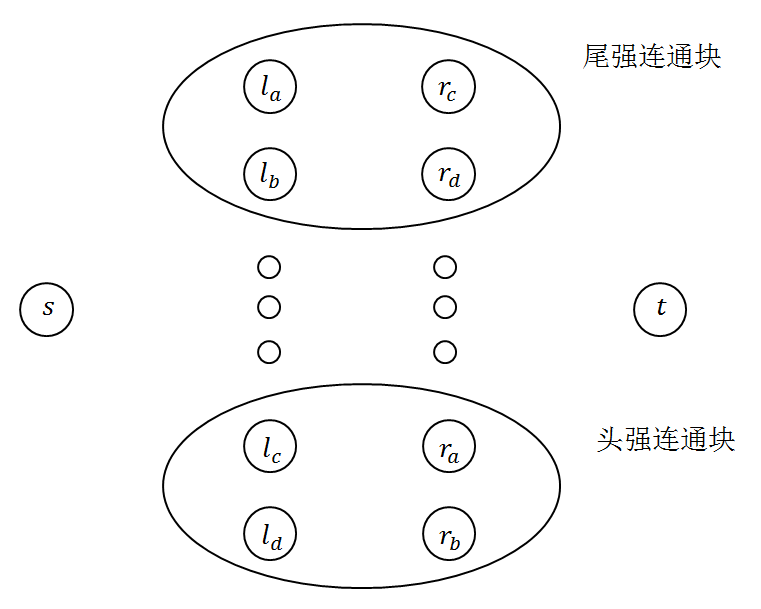
\includegraphics[width=0.65\textwidth]{eps/1.png}
    \caption{残余图中尾强连通分量与对应的头强连通分量}
    \label{fig:mesh1}
\end{figure}

\begin{claim} \label{residualgraph4}
在残余图$G_W(f)$中没有边从顶点集合$(L_W \cup R_W) \setminus (L_{N_G(T)} \cup R_T)$到顶点集合$L_{N_G(T)} \cup R_T$中。
\end{claim}
\begin{proof}
首先我们将残余图$G_W(f)$中
从顶点集合$L_{N_G(T)} \cup R_T$到顶点集合$(L_W \cup R_W) \setminus (L_{N_G(T)} \cup R_T)$中边分成两个集合,
注意在网络$W$中,排除$s, t$后,只有从$L_W$到$R_W$的边。
  \begin{equation*} \begin{aligned}
    & E_L = \{(u, v) \in E_W\;|\;u \in L_W \setminus L_{N_G(T)},v \in R_T\} \\
    & E_R = \{(v, u)\;|\;(u, v) \in E_W,f(u, v) > 0,u \in L_{N_G(T)},v \in R_W \setminus R_T\}
  \end{aligned} \end{equation*}

回顾定义\ref{NetworkDefintion},显然$E_L$为空集。
同时由于$\abs{R_T} = \abs{L_{N_G(T)}}$,且$E_L$为空,
所以所有从集合$L_{N_G(T)}$流出的流量都会流入集合$R_T$中,
因此$E_R$也是空集。

故,$E_L = E_R = \emptyset$,证毕。
\end{proof}



对于残余图$G_W(f)$的所有强连通分量,他们之间构成了拓扑关系。
而新的残余图$G_{W'}(f')$与之对比,移除掉的强连通分量要不就在拓扑关系的顶端(没有外部边可以到达顶点集合$L_{N_G(T)} \cup R_T$中)
要不就在拓扑关系的末端(顶点集合$L_T \cup R_{N_G(T)}$是一个尾强连通分量),
而对于剩余强连通分量,强连通性以及拓扑关系都没有受到影响!
因此只需要在求出残余图$G_W(f)$的所有强连通分量之后,利用逆拓扑顺序遍历每一个强连通分量$S_W$,
检查该强连通分量是否不存在未被标记移除的后代以及是否满足$S_L \cap S_R = \emptyset$,
如果两个条件都成立,则将顶点集合$L_T \cup R_{N_G(T)}$与顶点集合$L_T \cup R_{N_G(T)}$中的强连通分量都标记为移除即可。


至此我们给出了核心化算法阶段二的所有证明,下面分析时间复杂度。
在整个核心化算法阶段二,其中我们只需要构造一个残余图,求出该残余图的所有强连通分量,最后逆拓扑顺序遍历这些强连通分量。
显然每个步骤都是可以做到线性时间复杂度的,故整体时间复杂度为$O(\abs{V} + \abs{E})$。

\subsection{完整核心化算法}

伪代码详见Algorithm 1。

其中,我们将VCAL问题实例以及预先构造好的网络及其最大流作为输入,并且在核心化的过程中也将新图对应的网络及其最大流构造好并输出。


\begin{algorithm} 
\caption{完整核心化算法}
\begin{algorithmic}[1] 
\Require VCAL问题实例$(G,k)$, 图$G$对应的网络$W$及其最大流$f$
\Ensure  核心化后的VCAL问题实例$(G',k')$,图$G'$对应的网络$W'$及其最大流$f'$,被取进顶点覆盖的顶点集合$S_1$,
        ,被排除出顶点覆盖的顶点集合$S_0$
\algrule
\Function{Kernelise}{$G, k, W, f$}
    \State $S_0 \gets \emptyset$
    \State $S_1 \gets \emptyset$
    \State \Comment 核心化算法阶段一
    \State 根据网络$W$在最大可行流$f$,构造图$G$的Primal-$LPVC(G)$最优解$x$

    \State $G_1 \gets G[V^x_{1/2}],\;k_1 \gets k - \abs{V^x_1}$
    \State $S_1 \gets S_1 \cup V^x_1$
    \State $S_0 \gets S_0 \cup V^x_0$
    \State $W_1 \gets \text{从网络$W$中移除顶点集合}\{l_v, r_v | v \in V^x_1 \cup V^x_0\}\text{以及相关边}$
    \State $f_1 \gets \text{将流量函数$f$定义域限定到网络$W'$的边集上}$

    \State \Comment 核心化算法阶段二
    \State 构造网络$W_1$在最大可行流$f_1$下的流量残余图$G_{W_1}(f_1)$
    \State $K \gets \text{求解图$G_{W_1}(f_1) \setminus \{s, t\}$的所有强连通分量}$

    \For {按逆拓扑顺序遍历K中每一个强连通分量$T\in K$}
        \If {强连通分量$T$不存在未被标记的后代\; \textbf{and}\;$\{v\;|\;l_v \in T, r_v \in T\} = \emptyset$}
            \State $S_0 \gets S_0 \cup \{v\;|\;l_v \in T\}$
            \State $S_1 \gets S_1 \cup \{v\;|\;r_v \in T\}$
            \State 标记强连通分量T
        \EndIf
    \EndFor
    \State $G_2 \gets G \setminus (S_0 \cup S_1),\;k_2 \gets k - \abs{S_1}$
    \State $W_2 \gets \text{从网络$W$中移除顶点集合}\{l_v, r_v | v \in S_1 \cup S_0\}\text{以及相关边}$
    \State $f_2 \gets \text{将流量函数$f$定义域限定到网络$W_2$的边集上}$

    \State \Return $(G_2, k_2, W_2, f_2, S_1, S_0)$
\EndFunction
\end{algorithmic}
\end{algorithm} 
\section{VCAL分支算法}
上一章中,已经给出了基于线性松弛下界的参数化顶点覆盖问题(VCAL)的核心化算法,
将图G在线性时间内收缩至满足全$\frac{1}{2}$函数是其LPVC唯一最优解(即$surplus(G) \ge 1$)。
本章之中,我们将给出3条分支规则作用于核心化后的图上,
这些规则组成了本章的分支算法。
对于每一条分支规则,我们保证其都可以在线性时间内测试是否适用,并且如果决定执行,执行时间复杂度也是线性的。
最后证明在这些分支规则的共同作用下整棵搜索树的节点数量不超过$2.618^\mu$。

\vspace{0.5cm}
为了更好的分析分支算法的时间负责度,首先给出以下引理:
\begin{lemma} \label{LemmaUpdateMaxflow}
假设图G满足$surplus(G) \ge 1$,且对于求解Dual-$LPVC(G)$模型的网络W已经求得其最大流$f$。
令$G' = G \setminus S$,则可以在$O(\abs{S}(\abs{V} + \abs{E}))$的时间复杂度内
获得$G'$上求解Dual-$LPVC(G')$模型的网络$W'$上的最大流$f'$。
\end{lemma}

\begin{proof}
回顾\ref{TransformToNetwork}中内容,对于网络$W'$其有向图$G_{W'}$等价于有向图$G_W$移除顶点集合$L_S \cup R_S$以及相应的边集,即$G_{W'} = G_W \setminus \{L_S \cup R_S\}$。
因此如果网络W上一个可行流没有流量经过顶点集合$L_S \cup R_S$,则将其定义域限制为$E_{W'}$后便是网络$W'$上的可行流。

对网络W的最大流$f$进行退流操作,移除所有经过顶点集合$L_S \cup R_S$的流量,
因为在有向图$G_W$只有从$s$到$L_W$,从$L_W$到$R_W$以及从$R_W$到$t$的有向边,所以该操作可以在$O(\abs{V} + \abs{E})$的时间复杂度内完成。
将退流后的可行流流量函数定义域限定为$E_{W'}$,并命名为$f'$。显然$f'$是网络$W'$上的可行流。比较两个可行流的流量,
可以得$F' \ge F - 2 \abs{S}$。

对当前网络$W'$的可行流$f'$使用Ford-Fulkerson算法进行增广,假设增广$\Delta$流量后$f'$成为最大可行流,
则增广的时间复杂度是$O(\Delta(\abs{V} + \abs{E}))$。
因为网络$W'$中到达汇点t的边的容量和为$\abs{V'} = F - \abs{S}$,所以最大流流量$F' + \Delta \le F - \abs{S}$。
整理可以获得$\Delta \le \abs{S}$。综上,将可行流$f'$增广至最大流的时间复杂度为$O(\abs{S}(\abs{V} + \abs{E}))$。

证毕。
\end{proof}


\subsection{分支策略}
在分支算法开始之前,首先我们在图G中任意取一个顶点$v \in V$,
由于$surplus(G) \ge 1$,顶点$v$至少有两个邻居,取其中任意两个,记为$u_1, u_2$。


对于图G中的任何一个顶点覆盖,显然或者包含了顶点$v$, 或者同时包含了顶点$u_1, u_2$。
很自然,我们会考虑产生两个搜索分支,使得其中一个将顶点$v$取进顶点覆盖集合,另外一个将顶点$u_1, u_2$取进。
为了限制搜索树大小,这里我们增加了一个前提条件,
要求在图$G \setminus \{u_1, u_2\}$上全$\frac{1}{2}$函数是其Primal-$LPVC(G \setminus \{u_1, u_2\})$模型的最优解,
即$vc^*(G \setminus \{u_1, u_2\}) = (\abs{V} - 2) / 2$。\\

\begin{tabular}{ p{0.9\headwidth} }
  \hline
  \textbf{分支规则 一 }\\
  \textbf{前提:}  在图$G \setminus \{u_1, u_2\}$上,$vc^*(G \setminus \{u_1, u_2\}) = (\abs{V} - 2) / 2$\\
  \textbf{分支一:} $(G_1 \leftarrow G \setminus \{v\},\; k_1 \leftarrow k - 1)$\\
  \textbf{分支二:} $(G_2 \leftarrow G \setminus \{u_1, u_2\},\; k_2 \leftarrow k - 2)$\\
  \hline
\end{tabular} \vspace{0.5cm}

根据引理\ref{LemmaUpdateMaxflow},显然测试分支规则一的前提是否成立,更新分支一、分支二的问题实例的$LPVC$问题最优解均可以在线性时间内完成。

之后我们考虑分支规则一不被执行的情形,即发现$vc^*(G \setminus \{u_1, u_2\}) < (\abs{V} - 2) / 2$。
此时我们对于图$G \setminus \{u_1, u_2\}$执行\ref{KerneliseAlgorithm}节给出的核心化算法,
设$G'$为图$G\setminus\{u_1, u_2\}$收缩后得到的新图,且已经被核心化算法取进顶点覆盖集的顶点集合为$V_1 \subseteq V$,
已经被标记不属于定点覆盖集合的顶点集合为$V_0 \subseteq V$。

\begin{claim}
对于顶点集合$V_1$, $V_0$有
\begin{itemize}
  \item{(1)}$\abs{V_1} = \abs{V_0} - 1$;
  \item{(2)}顶点集合$V_0 \subseteq V$是图G的一个独立集,且$N_G(V_0) = V_1 \cup \{u_1, u_2\}$。
\end{itemize}
\end{claim}
\begin{proof}
(1)构造一个图$G\setminus\{u_1, u_2\}$上Primal-$LPVC(G\setminus\{u_1, u_2\})$模型的解$ : V \setminus \{u_1, u_2\} \rightarrow \{0, \frac{1}{2}, 1\}$如下,
\begin{equation*}
   \begin{cases}
            x^*_v =0, & \mbox{对于顶点$v \in V_0$;}  \\
            x^*_v =1, & \mbox{对于顶点$v \in V_1$;}  \\
            x^*_v =\frac{1}{2}, & \mbox{其他。}
          \end{cases}
\end{equation*}
由\ref{KerneliseAlgorithm}节给出的核心化算法定义,显然这样构造出来的$x^*$是Primal-$LPVC(G\setminus\{u_1, u_2\})$的最优解。
又因为此时分支规则一不能应用,可得:
$vc^*(G\setminus\{u_1, u_2\}) = val(x^*) = \abs{V_1} + (\abs{V} - \abs{V_1} - \abs{V_0} - 2) / 2 < (\abs{V} - 2) / 2$,
化简得:$\abs{V_1} < \abs{V_0}$。

构造一个图$G$上Primal-$LPVC(G)$模型的解$x : V \rightarrow \{0, \frac{1}{2}, 1\}$如下,
\begin{equation*}
   \begin{cases}
            x_v =0, & \mbox{对于顶点$v \in V_0$;}  \\
            x_v =1, & \mbox{对于顶点$v \in V_1 \cup \{u_1, u_2\}$;}  \\
            x_v =\frac{1}{2}, & \mbox{其他。}
          \end{cases}
\end{equation*}
又因为已知全$\frac{1}{2}$函数是其图$G$上Primal-$LPVC(G)$唯一最优解,可得,
$val(x) = \abs{V_1} + 2 + (\abs{V} - \abs{V_1} - \abs{V_0} - 2) / 2 \ge vc^*(G) + 1/2 = (\abs{V} + 1) / 2$。
化简得:$\abs{V_1} \ge \abs{V_0} - 1$。

综上有$\abs{V_1} = \abs{V_0} - 1$。

(2)$V_0$在图$G\setminus\{u_1, u_2\}$中是独立集,显然其在图G中也是独立集。
假设$u_1$或者$u_2$不在$N_G(V_0)$中,则有$surplus(G) \le surplus_G(V_0) \le \abs{V_1} + 1 - \abs{V_0} = 0$。
这与已知$surplus(G) \ge 1$矛盾。故$u_1,u_2 \in N_G(V_0)$,即$N_G(V_0) = V_1 \cup \{u_1, u_2\}$。

证毕。
\end{proof}

后面根据$V_1 \cup \{u_1, u_0\}$是否图$G$中的独立集进行分类讨论。
%为了后文描述更加清晰,此处将$V_1 \cup \{u_1, u_0\}$重新定义成$V_1$。

在$V_1 \cup \{u_1, u_0\}$不是图$G$中的一个独立集的情况下,应用分支规则二如下:\\

\begin{tabular}{ p{0.9\headwidth} }
  \hline
  \textbf{分支规则 二 }\\
  \textbf{前提:}  顶点集合$V_1 \cup \{u_1, u_0\}\subseteq V$不是图$G$中的一个独立集\\
  \textbf{分支一:} $(G_1 \leftarrow G \setminus (V_0 \cup V_1 \cup \{u_0, u_1\}),\; k_1 \leftarrow k - \abs{V_1} - 2)$\\
  \hline
\end{tabular} \vspace{0.5cm}

分支规则二实际上没有产生多个搜索分支,但是为了更方便分析搜索树大小这里将其归入其中。首先我们给出一个引理来证明它的正确性。
\begin{lemma} \label{SurplusOne1}
对于图$G(V, E)$,假设$surplus(G) \ge 1$且存在独立集$S \subseteq V$满足$surplus(S) = 1$和$N(S)$并不是独立集,
则存在一个图$G$的最小顶点覆盖,其包含所有$N(S)$中顶点且不包含所有$S$中顶点。
\end{lemma}
\begin{proof}
令$G' = G[S \cup N(S)]$,假设$vc(G')\le \abs{S}$。
令顶点集合$VC'$是图$G'$的最小顶点覆盖集之一,将其分解为$VC' = A \uplus B$,其中$A \subseteq S$且$B \subseteq N(S)$。

因为$G'$中不存在孤立点且S是独立集,所以$S$中不被$A$包含的顶点肯定每个都与集合$B$相邻,即$N(S \setminus A) \subseteq B$。
由$N(S)$并非图G中的一个独立集,可以得知$B \neq \emptyset$,再考虑$\abs{A} + \abs{B} = \abs{VC'} \le \abs{S}$,
故$\abs{A} < \abs{S}$,因此$S \setminus A$显然也非空。
考虑独立集$S \setminus A$的盈余值$surplus(S \setminus A) \le \abs{B} - (\abs{S \setminus A}) \le 0$,这与$surplus(G) \ge 1$矛盾。
所以$G'$的最小顶点覆盖集大小大于$\abs{S}$。

又因为我们可以获得一个大小为$\abs{S} + 1$的顶点覆盖集合($N(S)$就是这样一个顶点集合),综上$vc(G') = \abs{S} + 1$。

通过上文的图$G'$的构造我们知道任意图$G$的最小顶点覆盖至少包含$\abs{S} + 1$个集合$S \cup N(S)$中的顶点。
假设顶点集合$VC$是图$G$的一个最小顶点覆盖集,我们可以构造一个新的顶点集合如下$VC^* = VC \setminus (S \cup N(S)) \cup N(S)$。
显然$VC^*$也会是图$G$的一个顶点覆盖集合,并且它的大小不会超过$VC$。
综上$VC^*$是图$G$的最小顶点覆盖,其包含所有$N(S)$中顶点且不包含所有$S$中顶点。证毕。
\end{proof}

再回顾分支规则二,首先在我们应用分支规则的图$G$上有$surplus(G) \ge 1$,其次$V_0$是图G上盈余值为1的一个独立集,
最后我们只在$V_0$的邻居顶点集合$V_1 \cup \{u_1, u_2\}$不是独立集的前提下应用分支规则二。
所以,根据引理\ref{SurplusOne1},此时存在图$G$的最小顶点覆盖集合包含所有$V_1 \cup \{u_1, u_2\}$中顶点,且不包含所有$V_0$中顶点。
至此成功证明了分支规则二的正确性,我们可以在不能应用分支规则一并且$V_1 \cup \{u_1, u_2\}$不是图$G$中的一个独立集的情况下,
先将$V_1 \cup \{u_1, u_2\}$中顶点选进顶点覆盖集合中。

接下来分析分支规则二的时间复杂度。
显然应用核心化算法在图$G \setminus \{u_1, u_2\}$上,
和判断顶点集合$V_1 \cup \{u_1, u_2\}$是否图G中的独立集均可以在$O(\abs{V} + \abs{E})$时间负责度内完成。
对于分支规则二产生的图$G_1$,其等价于前文中我们对图$G \setminus \{u_1, u_2\}$应用核心化算法收缩出来的新图$G'$,
在核心化算法中,已经获得了其对应的求解Dual-$LPVC(G')$模型的网络的最大流。所以不需要额外时间复杂度去求解该网络的最大流,
故分支规则二,也可以在线性时间内应用。

最后讨论剩余的情况,此时$V_1 \cup \{u_1, u_2\}$是图$G$中的一个独立集。

因为$surplus_G(V_1 \cup \{u_1, u_2\}) \ge surplus(G) \ge 1$,所以独立集$V_1 \cup \{u_1, u_2\}$至少有两个邻居不在点集$V_0$中,
即在图$G'$上,保留其至少两个邻居,这里我们取其中任意两个,设为$u_1', u_2'$。\\

\begin{tabular}{ p{0.9\headwidth} }
  \hline
  \textbf{分支规则 三 }\\
  \textbf{前提:} 顶点集合$V_1 \cup \{u_1, u_0\}\subseteq V$是图$G$中的一个独立集 \\
  \textbf{分支一:} $(G_1 \leftarrow G',\; k_1 \leftarrow k - \abs{V_1} - 2)$\\
  \textbf{分支二:} $(G_2 \leftarrow G' \setminus \{u_1', u_2'\},\; k_2 \leftarrow k - \abs{V_0} - 2)$\\
  \hline
\end{tabular} \vspace{0.5cm}

为了证明分支规则三的正确性,同样我们此处也引进一个新的引理,如下:
\begin{lemma} \label{SurplusOne2}
  对于图$G(V, E)$,假设$surplus(G) \ge 1$且存在独立集$S \subseteq V$满足$surplus(S) = 1$和$N(S)$是独立集,
则或者存在一个图$G$的最小顶点覆盖,其包含所有$N(S)$中顶点;
或者与之相反,存在一个图$G$的最小顶点覆盖其不包含所有$N(S)$中顶点。
\end{lemma}
\begin{proof}
令顶点集合$VC$是图$G$的最小顶点覆盖集之一,将其分解为$VC = A \uplus B \uplus C$,
其中$A \subseteq S$,$B \subseteq N(S)$且$C \cap (S \cup N(S)) = \emptyset$。
显然当$A = \emptyset$时,$B = N(S)$;当时$B = \emptyset$时,$A = S$。
因此我们只需要证明当顶点集合$A,B$同时非空时,可以构造出一新的图$G$的最小顶点覆盖使得其中一个集合为空。

假设顶点集合$A,B$同时非空。同理于引理\ref{SurplusOne1}的证明,可以得知此时$\abs{A} + \abs{B} \ge \abs{S} + 1$。
构造一新的顶点集合$VC' = N(S) \cup C$,显然$VC'$是图G的一个顶点覆盖,又因为$\abs{VC'} = \abs{C} + \abs{S} + 1 \le \abs{A} + \abs{B} + \abs{C} = \abs{VC}$,
所以它也是图G的一个最小顶点覆盖。

证毕。
\end{proof}

考虑在分支规则一与分支规则二均不能应用的情况下,
首先在我们应用分支规则的图$G$上已经有了$surplus(G) \ge 1$;
其次当分支规则一不能应用时候,$V_0$是图G上盈余值为1的一个独立集;
最后当分支规则二不能应用时候,$V_0$的邻居顶点集合$V_1 \cup \{u_1, u_2\}$是图$G$的一个独立集。
所以依据引理\ref{SurplusOne2},此时我们可以将原问题实例分成两个分支,
其中一个将顶点集合$V_1 \cup \{u_1, u_2\}$先取进顶点覆盖集,
另外一个将顶点集合$V_1 \cup \{u_1, u_2\}$的邻居先取进顶点覆盖集合。至此我们成功证明了分支规则三的正确性。

接下来我们分析执行分支规则三的时间复杂度。
根据我们的分类讨论情形,当分支规则一和二不能执行的时候,总会执行分支规则三,因此不需要额外测试是否执行该规则。
在利用核心化算法构造$G'$的时候,已经求得其Dual-$LPVC(G')$模型的最优解。
同时依据引理\ref{LemmaUpdateMaxflow},可以在求解Dual-$LPVC(G')$模型的网络的最大可行流的基础上,
在$O(2(\abs{V} + \abs{E}))$的时间负责度内构造分支二的对应的最大可行流。
故,分支规则三也能在线性时间复杂度内被执行。

\subsection{算法时间复杂度分析}
在上一节中,我们已经给出了3个分支规则,并且证明每个规则的正确性以及保证他们都能在线性时间内被执行。
接下来只剩下讨论搜索树大小。这里我们利用参数$u$的下降来进行分析。

对于我们核心化算法来说,在给出的时候已经证明其保证收缩后的VCAL问题实例$(G', k')$相比原来的VCAL问题实例$(G, k)$,有:
$\mu(G', k') \le \mu(G,  k)$。现在讨论每个分支规则应用后产生的每个分支的问题实例的参数,对比应用前的参数的变化。

\vspace{0.5cm}

首先回顾上一节给出的分支规则一。
我们通过或者使顶点覆盖集合包含顶点$v$, 或者使顶点覆盖集合包含顶点$u_1, u_2$,在原来VCAL问题实例的基础上产生了两个搜索分支。
这里对每个分支上的新问题实例的参数分别进行分析。

对于分支一,由于$surplus(G) \ge 1$,所以删除掉一个顶点后的图$G_1$上有$surplus(G_1) \ge 0$。
根据引理\ref{relationBwtSurplusAndLPVC},可以得知全$\frac{1}{2}$函数是图$G_1$上的Primal-$LPVC(G_1)$模型的最优解,即$vc^*(G_1) = \frac{\abs{V} - 1}{2}$。
所以有$\mu(G_1, k_1) = k_1 - vc^*(G_1) = k - 1 - \frac{\abs{V} - 1}{2} = \mu(G, k) - \frac{1}{2}$。

对于分支二,由分支规则一应用的前提可以得知$vc^*(G_2) = \frac{\abs{V} - 2}{2}$。
所以有$\mu(G_2, k_2) = k_2 - vc^*(G_2) = k - 2 - \frac{\abs{V} - 2}{2} = \mu(G, k) - 1$。

综上,这里更新分支规则一的描述,如下:\\

\begin{tabular}{ p{0.12\headwidth} | p{0.12\headwidth}p{0.66\headwidth} }
  \multicolumn{3}{l}{ \textbf{分支规则 一:} }\\
  \hline
  \textbf{前提:}  & \multicolumn{2}{l}{在图$G \setminus \{u_1, u_2\}$上,$vc^*(G \setminus \{u_1, u_2\}) = (\abs{V} - 2) / 2$}\\
  \hline
  \textbf{分支一:} & 问题实例:&$(G_1 \leftarrow G \setminus \{v\},\; k_1 \leftarrow k - 1)$ \\
                    & 参数:&$\mu(G_1, k_1) = \mu(G, k) - \frac{1}{2}$\\
  \hline
  \textbf{分支二:} & 问题实例:&$(G_2 \leftarrow G \setminus \{u_1, u_2\},\; k_2 \leftarrow k - 2)$\\
                    & 参数:&$\mu(G_2, k_2) = \mu(G, k) - 1$\\
  \hline
\end{tabular} \vspace{0.5cm}  

\vspace{0.5cm}
再考虑分支规则二。当分支规则一不能执行的时候,我们利用核心化算法对图$G \setminus \{u_1, u_2\}$进行收缩。
获得了算法收缩后的新图$G'$,被算法取进该图顶点覆盖集的顶点集合$V_1$以及被算法排除出该图顶点覆盖集合的顶点集合$V_0$。
而当顶点集合$V_1 \cup \{u_1, u_2\}$不是图G的独立集时候,我们应用分支规则二,产生了一个新的搜索分支。

对于分支规则二产生的唯一搜索分支,由于应用核心化算法得到的新图$G'$满足全$\frac{1}{2}$函数是图$G'$上的Primal-$LPVC(G')$模型的唯一最优解,
所以$vc^*(G_1) = \frac{\abs{V} - \abs{V_0} - \abs{V_1} - 2}{2}$。
另外已经证明了$\abs{V_1} = \abs{V_0} - 1$。故,
\begin{equation*} \begin{aligned}
    \mu(G_1, k_1) & = k_1 - vc^*(G_1)  \\
                  & = k_1 - \abs{V_1} - 2 - \frac{\abs{V} - \abs{V_0} - \abs{V_1} - 2}{2} \\
                  & = k_1 - (\abs{V_0} - 1) - 2 - \frac{\abs{V} - \abs{V_0} - (\abs{V_0} - 1) - 2}{2} \\
                  & = k - \frac{\abs{V}}{2} - \frac{1}{2} = \mu(G, k) - \frac{1}{2}
\end{aligned} \end{equation*}
更新分支规则二描述,如下;\\

\begin{tabular}{ p{0.12\headwidth} | p{0.12\headwidth}p{0.66\headwidth} }
  \multicolumn{3}{l}{ \textbf{分支规则 二:} }\\
  \hline
  \textbf{前提:}  & \multicolumn{2}{l}{顶点集合$V_1 \cup \{u_1, u_0\}\subseteq V$不是图$G$中的一个独立集}\\
  \hline
  \textbf{分支一:} & 问题实例:&$(G_1 \leftarrow G \setminus (V_0 \cup V_1 \cup \{u_0, u_1\}),\; k_1 \leftarrow k - \abs{V_1} - 2)$ \\
                    & 参数:&$\mu(G_1, k_1) = \mu(G, k) - \frac{1}{2}$\\
  \hline
\end{tabular} \vspace{0.5cm}  

\vspace{0.5cm}
最后看回分支规则三。当分支规则一和二不满足应用条件的时候,该分支规则会被应用,并且类似规则一,也会分裂出两个新的搜索分支。
对于分支一,同理于分支规则二的分支,可以得知$\mu(G_1, k_1) = \mu(G, k) - \frac{1}{2}$。
对于分支二,我们先证明以下断言:
\begin{claim}
全$\frac{1}{2}$函数是图$G_2$上Primal-$LPVC(G_2)$模型的最优解,即$surplus(G_2) \ge 0$。
\end{claim}
\begin{proof}
假设该断言不成立,即存在一个图$G_2$上的独立集满足$surplus_{G_2}(S) < 0$。
显然顶点集合$S \cup V_0 \subseteq V$,是图G上的一个独立集,
其在图G上的盈余值如下,
\begin{equation*} \begin{aligned}
  surplus_G(S \cup V_1) &\le surplus_{G_2}(S) + \abs{V_1}  - \abs{V_0} + 2 \\
                        &= surplus_{G_2}(S) + 1 \le 0
\end{aligned} \end{equation*}
\end{proof}


\section{小结}

\cleardoublepage
\chapter{反馈顶点集问题的固定参数算法}
反馈顶点集问题(Feedback Vertex Set, 缩写为FVS),即对于参数k,询问给定图中是否存在大小满足k的顶点集合满足:
对于图中任意一条环都与这个顶点集有交集。
与顶点覆盖问题类似,该问题也是最早被提出来的21个NP-complete问题之一\cite{karp1972reducibility}。

本章提出了一个时间复杂度为$\mathcal{O}(2.554^k)$的固定参数算法。
\section{相关术语及问题的定义}

本章里我们会继续沿用上一大章中关于图的符号和术语。同时,在本节中我们会继续扩充一些会使用到的术语,
并且给出相关问题更加具体的数学的定义。
\subsection{有关图的一些术语的定义}
首先给出无向图上一些常见名词的定义,如环,树和森林等。
\begin{definition}[环]
对于无向图$G(V,E)$,假设存在一个顶点序列$v_1v_2...v_n$,使得$\{v_0, v_n\} \in E$并且对于任意$0 \le i < n$有$\{v_i, v_{i+1}\} \in E$。
则该序列为图G上的一个\textbf{环}。如果该序列中没有重复顶点,则称之为图G的一个\textbf{简单环}。
\end{definition}

\begin{definition}[树(tree)和森林(forest)]
对于无向图$G(V,E)$,如果其中不存在任何环,则我们称图G为一个\textbf{森林(forest)}。
同时如果图G是联通的,则其也被称为\textbf{树(tree)}。
\end{definition}

\begin{definition}[反馈顶点集]
对于图$G(V, E)$, 若集合$V' \subseteq V$使得$G \setminus V'$中不存在任何环(即,图$G \setminus V'$是森林),
则称$V'$是图G的一个\textbf{反馈顶点集}(Feedback Vertex Set, 简称$FVS$)。
\end{definition}

为了方面对于算法的描述,我们继续引进一些图的术语。对于图G,$cc(G)$表示图G上连通块的个数。

\subsection{参数化反馈顶点集问题}
对于一般图来说,回答是否存在大小不超过k的反馈顶点集,是非常经典组合优化问题。
在该问题上,固定参数算法是常用来求解答案的方法。
具体参数化反馈顶点集问题表述如下:\\

\begin{tabular}{| p{0.9\headwidth} |}
  \hline
  参数化反馈顶点集问题(Feedback Vertex Set,简称FVS) \\
  \textbf{输入:} 图$G(V, E)$及整数k \\
  \textbf{参数:} $k$\\
  \textbf{问题:} 图G中是否存在一个反馈顶点集合,其大小不超过k\\
  \hline
\end{tabular} \vspace{0.5cm} \\

在参数计算领域,参数化FVS也是其中一个非常重要的问题,
一系列的研究一直在不停的改进其下限,如文献\cite{bodlaender1994disjoint,downey1992fixed,downey2012parameterized,raman2006faster,kanj2004parameterized,dehne20072o,guo2006compression,chen2008improved,cao2010feedback,cygan2011solving,kociumaka2014faster} 等。

在文献\cite{cygan2011solving}中作者Cygan等利用其发明的Cut\&Count技术,设计了时间复杂度为$\mathcal{O}(3^k)$的固定参数算法来求解FVC问题。
该算法是一个蒙地卡罗算法(Monte Carlo algorithm),如果不存在大小不超过k的FVS集合,那么算法一定会返回“NO”,否则有1/2概率返回“YES”。
据我们所知,该算法是迄今为止FVS问题上复杂度最低的固定参数算法。
而如果不希望使用随机性算法的话,迄今最快的算法是Kociumaka等\upcite{kociumaka2014faster}在2014年提出的基于迭代压缩技术的算法,
他们可以在$\mathcal{O}(3.619^k)$的时间复杂度内确切的给出问题的答案。

本章中,我们同样使用迭代压缩技术,最后获得一个\textcolor[rgb]{1.00,0.00,0.00}{$\mathcal{O}(2.554^k)$}时间复杂度的固定参数算法。


\section{使用迭代压缩技术转化FVS问题}
与近年来大多数FVS问题的参数算法相似,我们首先基于迭代压缩技术将FVS问题转化成另外一个与之高度相关的问题,
Disjoint-FVS问题(Disjoint Feedback Vertex Set)。下面,给出Disjoint-FVS问题的详细定义:\\

\begin{tabular}{ | p{0.06\headwidth} p{0.80\headwidth} | }
  \hline
  \multicolumn{2}{|l|}{ \textbf{不相交反馈顶点集问题} }\\
  \multicolumn{2}{|l|}{ (Disjoint Feedback Vertex Set,简称Disjoint-FVS)}\\
  \textbf{输入:} & 图$G(V, E)$,整数k 以及顶点集合$V$的划分$V = U \uplus D$满足$G[U]$和$G[D]$都是森林\\
  \textbf{问题:} & 图$G$中是否存在一个反馈顶点集合$X \subseteq D$,其大小不超过k\\
  \hline
\end{tabular} \vspace{0.5cm}

首先,我们直接给出关于Disjoint-FVS问题的时间复杂度,并基于该结论和迭代压缩技术,给出FVS问题的时间复杂度。
之后,本章的剩余部分将注意力集中在Disjoint-FVS问题上,证明下述结论的正确性。
\begin{theorem} \label{Disjoint-FVSTime}
  对于一个Disjoint-FVS问题实例$I = (G, U, D, k)$,可以在$\mathcal{O}^*(C^k_{k + cc(G[U])/2})$时间复杂度内构成出符合条件的反馈顶点集合或者回答不存在这样的反馈顶点集合。
\end{theorem}

在定理\ref{Disjoint-FVSTime}中,我们使用了组合计数的方式来表达其复杂度,不过这并不是最终结果。
在后续应用中,我们只处理参数k与图$G[U]$连通块个数成一定比例的Disjoint-FVS问题实例,在这样情况下可以使用Stirling公式将其化简成$c^k$形式。

在定理\ref{Disjoint-FVSTime}的基础上,我们应用迭代压缩技术构造出下面求解FVS问题的算法。
\begin{theorem}
对于一个FVS问题实例$I = (G, k)$, 可以在可以在$\mathcal{O}^*(3.598^k)$时间复杂度内构成出大小不超过k的反馈顶点集合或者回答不存在这样的反馈定点集合。
\end{theorem}
\begin{proof}
令$v_1, v_2, ..., v_n$是图$G$顶点集合$V$的任意排列,对于$1 \le i \le n$定义顶点集合$V_i = \{v_1, v_2, ..., v_i\}$和图$G_i = G[V_i]$。
我们依次求解FVS问题实例$(G_i, k)$对于$i = k+1, ..., n$(注意:对于图$G_k$顶点集合$V_k$显然是反馈顶点集,不需要求解)。
显然如果对于某个i,FVS问题实例$(G_i, k)$无解,那么原问题实例$I$也无解,因为图$G_i$是图$G$的一个导出子图。

如果我们已经获得图$G_i$上大小不超过k的反馈顶点集合$X_i$,那么集合$X_i \cup \{v_{i+1}\}$则构成了图$G_{i+1}$的一个大小不超过k+1反馈顶点集合。
令$Z = X_i \cup \{v_{i+1}\}, D = V_i \setminus X_i = V_{i+1} \setminus Z$。
由定义可知$G_{i+1}[D] = G_i[D]$是一个森林。

接下来,我们枚举集合$Z$的所有子集$Y$,尝试回答当图$G_{i+1}$的反馈顶点集一定包含所有Y中顶点,并且一定不包含$Z \setminus Y$中顶点时,
其大小是否能够不超过k。令$U = Z \setminus Y$,显然当$G[U]$不是一个森林时,肯定不存在符合要求的反馈顶点集,因此我们后续只讨论$G[U]$是森林的情况。
此时根据上述约束,我们可以把当前的问题转换成Disjoint-FVS问题实例$I_Y = (G_{i+1} \setminus Y, U, D, k-\abs{Y})$。
由定理\ref{Disjoint-FVSTime},可以得知求解问题实例$I_Y$的时间复杂度为$\mathcal{O}^*(C^k_{k + cc(G[U])/2})$,其中$cc(G[U]) \le \abs{U} = k - \abs{Y}$,
故时间复杂度可以化简成,$\mathcal{O}^*(C^{k - \abs{Y}}_{3(k - \abs{Y})})$。
应用Stirling公式,可以得到,$\mathcal{O}^*(C^{k - \abs{Y}}_{3(k - \abs{Y})}) = \mathcal{O}^*(1.61185^{k - \abs{Y}})$。
最后,如果对于某个子集$Y \subseteq Z$,我们求解出Disjoint-FVS问题实例$I_Y$的反馈顶点集$X$,则$X \cup Y$是问题实例$(G_{i+1}, k)$的解。
反之,如果不存在这样的子集,那么问题实例$(G_{i+1}, k)$不存在解。

考虑整个过程的运行时间,求解问题实例$(G_{i+1}, k)$时间复杂度,如下:
\begin{equation*}
  \mathcal{O}^*(\sum_{Y \subseteq Z}C^{k - \abs{Y}}_{3(k - \abs{Y})}) \\
   = \mathcal{O}^*(\sum_{Y \subseteq Z}1.61185^{k - \abs{Y}})
   = \mathcal{O}^*((1 + 1.61185^2)^k) = \mathcal{O}^*(3.598^k)
\end{equation*}
从$G_{k+1}$到$G_n$,我们重复上述过程n - k次便可以求解原FVS问题实例$(G, k)$,整个过程时间复杂度也可以表示成$\mathcal{O}^*(3.598^k)$。

证毕。
\end{proof}

\section{Disjoint-FVS问题算法}
求解Disjoint-FVS问题的方法,一般都是分支限界法,基本思路是取出顶点集合D中的某个顶点v,通过假设v是否存在最终的反馈顶点集合,我们可以获得实例的两个分支。
本章中,我们将给出一个Disjoint-FVS问题的算法,以证明定理\ref{Disjoint-FVSTime}的正确性。

\subsection{Disjoint-FVS问题实例的评估}
我们的算法与之前Cao\upcite{cao2010feedback}和Kociumaka\upcite{kociumaka2014faster}的算法相似,
与这两个算法相比,我们创新性地使用一个二元组来评估Disjoint-FVS问题实例的复杂程度(改变使用单个数值来评估的方式)。
这在以前的参数算法文献中,也是十分罕见的。本节中,我们将给出具体的评估方法以及对其边界的证明。

首先,得益于前人的工作成果\upcite{cao2010feedback},我们知道某些情况下Disjoint-FVS问题是存在多项式解法的,
对于这部分满足条件的顶点,我们并不需要对进行枚举,而是可以在枚举完所有其他顶点后,直接在多项式时间内求解剩余问题。
下面,我们引入其中一个算法,如下:
\begin{lemma} \label{Disjoint-FVSSolvable}
对于一个Disjoint-FVS问题实例$(G, U, D, k)$,如果所有的顶点$v \in D$,满足其邻居数量$\abs{N(v)} \le 3$,
那么存在一个时间复杂度为$O(n^2log^6n)$的多项式算法,或者构造出图G的反馈顶点集$X$满足$\abs{X} \le k$并且$X \subseteq D$,
或者回答不存在这样的反馈顶点集。
\end{lemma}

定义顶点集合$T = \{v \in D\;|\;\abs{N(v)} = 3 \text{ 并且 } N(v) \subseteq U\}$。
根据引理\ref{Disjoint-FVSSolvable},我们并不需要对顶点集合T中的顶点进行枚举。
接下来,给出一个引理对顶点集合T的大小进行分析。

\begin{lemma}
对于Disjoint-FVS问题实例$I(G, U, D, k)$,如果$k + \frac{cc(G[U])}{2} - \abs{T} < 0$那么该实例肯定没有符合条件的解。
\end{lemma}

\begin{proof}
我们通过证明该命题的逆反命题,来证明引理的正确性。

假设顶点集合X是图G的一个反馈顶点集合,并且$X \subseteq D, \abs{X} \le k$,即问题实例I存在符合条件的解X。
则对于任意顶点$v \in (T \setminus X)$,v连接了3个不同的$G[U]$的连通块,所以$cc(G[U]) \ge 2\abs{T\setminus X} + 1$。
结合$\abs{X} \le k$, 可以获得,$\abs{T} = \abs{X \cap T} + \abs{T \setminus X} < k + \frac{cc(G[U])}{2}$。

证毕。
\end{proof}

\begin{definition}
对于Disjoint-FVS问题实例$I(G, U, D, k)$,定义其评估函数如下,
\[\mu(I) = (\mu_1(I), \mu_2(I)) = (k, k + \frac{1}{2}cc(G[U]) - \abs{T})\]
\end{definition}

显然,对于该评估函数,当$\mu_1(I) \le  0$或者$\mu_2(I) \le 0$的时候,问题实例多项式可解。
当$\mu_2(I) < 0$时,根据引理\ref{Disjoint-FVSSolvable},直接返回不存在符合条件的解;
当$\mu_1(I) = 0$时,那么检查图G是否森林就可以立刻返回答案。

\subsection{收缩规则}
本节中,我们给出若干特殊情况下,应用在Disjoint-FVS问题实例上的收缩规则,并且证明他们是安全且有效的。
假设对于一个收缩规则,将问题实例I转化成问题实例$I'$,我们说该规则是安全的,代表新问题实例$I'$有解当且仅当原问题实例I有解;
说该规则是有效的,则意味着其两个评估参数都没有上升,即$u_1(I') \le u_1(i), u_2(I') \le u_2(I)$。 \\

\begin{reducerule}
移除图G中所有度数为1的顶点。
\end{reducerule}

\begin{reducerule}
如果存在一个顶点$v \in D$,其有两个邻居在图$G[U]$的同一个连通块中,则移除顶点v并令k减少1, 即令$G \leftarrow G \setminus v, k \leftarrow k - 1$。
\end{reducerule}

\begin{reducerule}
如果存在一个顶点$v \in D$,其度数为2且至少有一个邻居在$U$中,则将其从顶点集合D中移到顶点集合U中,即令$U \leftarrow U \setminus \{v\}, D \leftarrow D \cup \{v\}$。
\end{reducerule}

\begin{reducerule}
如果存在一个顶点$v \in D$,其度数为2,则其删除并且在它的两个邻居间连一条边,即令$G \leftarrow G \setminus \{v\}, E(G) \leftarrow E(G) \cup N(v)$。
\end{reducerule}


\begin{reducerule}
如果存在一个度数为3的顶点$v \in D$,满足$\abs{D \cap N(v)} = 1$,
假设其3个顶点分别为$w \in D, u_1 \in U, u_2 \in U$,
删除顶点$v$和$w$之间的边,添加新顶点$z$属于顶点集合$U$,并且连接其与顶点$w$和$v$,
即令$Z \leftarrow Z \cup \{z\}, E(G) \leftarrow E(G) \cup \{e_{zw}, e_{zv}\} \setminus \{e_{wv}\}$。
\end{reducerule}


对于每个问题实例,我们按照给出顺序依次应用这个五个收缩规则,直到没有规则适用。
显然,这五条收缩规则都可以在多项式时间内应用,并且由于每次应用都会导致问题实例的规模的收缩,因此整个过程也是多项式的。
接下来,我们证明他们都是安全且有效的。

\begin{lemma}
收缩规则 1-5都是安全且有效的。
\end{lemma}
\begin{proof}
对于收缩规则1,度数为1的顶点不可能存在与任何环,可以直接忽略;
对于收缩规则2,如果不将顶点v取进反馈顶点集中,则剩余图必然存在环。
而在规则3、4中,我们可以证明假设存在一个满足问题实例$I(G, U, D, k)$的反馈顶点集X包含顶点v,那么一定可以构造另外一个符合条件的反馈顶点集$X'$不包含顶点v。
假设图$G \setminus (X \setminus \{v\})$中存在环(否则可以令$X' = X \setminus \{v\}$),
因为顶点v度数为2且其邻居不属于同一个$G[U]$连通块,所以环仅有一个并且环上一定有顶点不属于$U$,我们取其中一个记为$u$。
构造$X' = X \setminus \{v\} \cup \{u\}$,显然符合要求。因此这4条规则都是安全的。

对于这4条规则,显然k和$cc(G[U])$都不会上升。而集合T缩小只可能发生在规则1删除一个属于U的顶点时,此时$cc(G[U])$减少了1。因此这4条规则都是有效的。

最后讨论收缩规则5,收缩规则5使得新的问题实例增加了一个顶点$z \in U$,然而并没有增加任何新的环。
可以观察到如果新图上的环经过顶点$z$,那么这个环在原图上也存在,其经过了边$e_{wv}$。
因此,在这两个问题实例上求解反馈顶点集实际上是等价的,即规则5是安全的。
观察收缩规则5在创造一个新的图$cc(G[U])$的连通块的同时,令顶点$v$满足$abs{N(v)} = 3$并且$N(v) \subseteq U$,因此顶点集合$T$也增加了1。
故,应用完收缩规则5有,$u(I') = (k, u_b(I) + 1/2 - 1) = u(I) - (0, 1/2)$。因此收缩规则5也是安全有效的。

证毕。
\end{proof}


\subsection{分支规则}
前文已经提到,我们的算法是基于分支搜索的,每次会从顶点集合D中取出一个顶点,通过假设它存在最终的反馈顶点集或者不存在来获得两个搜索分支。
为了获得更加优秀运行时间上界,我们希望通过选择最合适的顶点,以提高评估函数$\mu(I)$的下降程度。
本节中我们首先给出合适的选择顶点的方法,并且对应用分支规则后的两个问题实例的评估函数变化进行分析。 

\begin{lemma}
对于Disjoint-FVS问题实例$I(G,U,D,k)$,当收缩规则1-5都不能应用且顶点集合$D \setminus T$非空时,
至少存在顶点$v \in (D \setminus T)$,其邻居中至少有3个顶点在集合U。
\end{lemma}
\begin{proof}
首先,收缩规则1-5都不能应用可以推导出D中所有顶点度数都大于等于3。
其次顶点集合$D \setminus T$的导出子图是森林,取森林的任意孤立节点或者叶子结点v,顶点v满足$\abs{N(v) \cap D} \le 1$。
再结合顶点v不满足收缩规则5的应用条件,可以得知顶点v至少有3个邻居在U中。
\end{proof}

根据上述引理,我们总能应用以下分支规则。\\

\begin{tabular}{ p{0.9\headwidth} }
  \hline
  \textbf{分支规则}\\
  \textbf{前提:} 存在一个顶点$v \in (D \setminus T)$,其邻居中至少有3个顶点在集合U内。\\
  \textbf{分支一:} $(G_1 \leftarrow G \setminus \{v\},\; U_1 \leftarrow U,\; D_1 \leftarrow D \setminus \{v\}, k_1 \leftarrow k - 1)$\\
  \textbf{分支二:} $(G_2 \leftarrow G,\; U_2 \leftarrow U \cup \{v\},\; D_2 \leftarrow D \setminus \{v\}, k_2 \leftarrow k)$\\
  \hline
\end{tabular} \vspace{0.5cm}

对于分支一,我们将顶点v取进了反馈顶点集,即可以获得一个不包含顶点v的新问题实例$I_1$,此时$k_1$减少1,同时$cc(G_1[U_1])$和$\abs{T_1}$显然没有发生任何变化。
因此,
\begin{equation*}
  \begin{aligned}
    & u_a(I_1) = k - 1 = u_a(I) - 1 \\
    & u_b(I_1) = k - 1 + \frac{1}{2}cc(G[U]) - \abs{T} = u_b(I) - 1
  \end{aligned}
\end{equation*}
而对于分支二,当我们决定将顶点v排除出反馈顶点集时,可以将其移动到集合U中,由于收缩规则2不能被应用,
顶点v的所有邻居处于不同的$G[U]$连通块中,因此$G[U_2]$依然是森林并且$cc(G[U_2]) \le cc(G[U]) - 2$。同时此时$k$保持不变,$\abs{T}$有可能增加但不可能减少。
因此有,
\begin{equation*}
  \begin{aligned}
    & u_a(I_2) = u_a(I) \\
    & u_b(I_2) \le k + \frac{1}{2}(cc(G[U]) - 1) - \abs{T} = u_b(I) - 1
  \end{aligned}
\end{equation*}

\subsection{复杂度分析}
对于Disjoint-FVS问题实例,假设函数$T(\mu(I))$表示其搜索树节点个数。
回顾上一节的分支规则,其产生两个搜索分支,我们已经分析了其评估函数的变化,因此对于当前问题实例的搜索树规模,有
\begin{equation*} \begin{aligned}
  T(\mu(I)) & = T(\mu_a(I), \mu_b(I)) \\
            & \le T(\mu_a(I) - 1,\; \mu_b(I) - 1) +  T(\mu_a(I),\; \mu_b(I) - 1)
\end{aligned} \end{equation*}
此外,之前也讨论了当$\mu_a \le 0$或者$\mu_b \le 0$时,$T(\mu) = 1$。因此,我们可以得知
\[T(\mu(I)) \le C^{\mu_a}_{\mu_b} \le C^k_{k + cc(G[U])/2}\]
因此对于任何Disjoint-FVS问题实例,可以在$\mathcal{O}(C^k_{k + cc(G[U])/2})$时间复杂度内构成出符合条件的反馈顶点集合或者回答不存在这样的反馈顶定集合。
至此我们成功证明了引理\ref{Disjoint-FVSTime}。


\section{小结}

在本节中我们首先给出本章算法的伪代码,如下。

我们将算法分解成两个函数。首先给出Disjoint-FVS算法,如\ref{disjoint-fvs-algorithm}节所描述的这是一个分支搜索算法。
每次进入递归函数,首先应用收缩规则进行收缩,之后如果程序没有到达多项式可解或者到达不可能存在合法解的情形,我们选取顶点并进行分支搜索。具体伪代码,如下:\\

\begin{algorithm}
\caption{Disjoint-FVS算法}
\begin{algorithmic}[1]
\Require Disjoint问题实例$(G,U, D, k)$
\Ensure  符合条件的问题实例反馈顶点集合或者 “NO”
\algrule
\Function{Disjoint-FVS}{$G, U, D, k$}
    \State $G, U, D, k \gets ApplyReduceRlues(G, U, D, k)$ \Comment 首先应用收缩规则1-5
    \State $T \gets \{v \in D\;|\;\abs{N(v)} = 3 \text{ and } N(v) \subseteq U\}$
    \State $u_a \gets k, u_b \gets k + \frac{1}{2}cc(G[U]) - \abs{T}$
    \State \textbf{if} ($u_a < 0$) or ($u_b < 0$) \textbf{then} \Return "NO" \Comment 搜索终止条件,已经不可能存在解
    \If {$D = T$ }
        \State 在多项式时间内求解当前问题并返回结果 \Comment 引理\ref{Disjoint-FVSSolvable}
    \Else
        \State 取$D$中至少有3个邻居在$U$中的任一顶点$v$
        \State \Comment 引理\ref{vertexNDge3}表明这样的顶点一定存在
        \State $branchA \gets \text{Disjoint-FVS}(G \setminus v, U, D \setminus v, k - 1)$
        \Comment 分支1: $v \in FVS$
        \State \textbf{if} branchA不等于“NO” \textbf{then} \Return $branchA \cup \{v\}$
        \State \Return \text{Disjoint-FVS}$(G, U\cup\{v\}, D \setminus v, k)$
        \Comment 分支2: $v \notin FVS$
    \EndIf
\EndFunction
\end{algorithmic}
\end{algorithm}

\newpage
最后是完整的FVS问题算法,如前文所述其中我们使用了迭代压缩技术,通过依次加入每个顶点来最终求解完整问题实例。
期间,我们枚举完当前顶点覆盖集$Z$的子集后会构造Disjoint-FVS问题实例并会调用前面的Disjoint-FVS算法。
具体伪代码,如下:\\

\begin{algorithm}
\caption{FVS算法}
\begin{algorithmic}[1]
\Require FVS问题实例$(G,k)$
\Ensure  符合条件的问题实例反馈顶点集合或者 “NO”
\algrule
\Function{FVS}{$G, k$}
    \State $V_i \gets \emptyset, X \gets \emptyset$
    \For {遍历所有顶点$v\in V$}
        \State $V_i \gets V_i \cup v, G_i \gets G[V_i], D \gets V_i \setminus X$
        \State $Z \gets X \cup \{v\}$
        \State \textbf{If} $\abs{Z} \le k$ \textbf{then} 令$X \gets Z$并且\textbf{continue}
        \For {遍历所有$Z$的子集$Y \subseteq Z$}
            \State \textbf{If} $G[Z \setminus Y]$不是森林 \textbf{then} \textbf{continue}
            \State $result \gets \text{Disjoint-FVS}(G_i \setminus Y, Z \setminus Y, D, k - \abs{Y})$
            \State \textbf{If} $result$不是“NO” \textbf{then} 令$X \gets Y \cup result$并且\textbf{break}
        \EndFor
        \State \textbf{If} 对于所有$Z$的子集$result$均是“NO” \textbf{then} \Return “NO”
    \EndFor
    \State \Return X
\EndFunction
\end{algorithmic}
\end{algorithm}

至此,本章中完整地给出了一个求解经典参数化反馈顶点集问题的确定性固定参数算法,
时间复杂度为$\mathcal{O}^*(3.598)$。


\cleardoublepage
\chapter{总结与展望}

本章总结全文的工作,并对展望未来的研究前景和进一步努力的方向。

\section{工作总结}
本文主要从参数计算与复杂性理论的角度研究NP-hard问题。
具体的研究对象有基于线性松弛下界的参数化顶点覆盖问题和参数化反馈顶点集问题。
顶点覆盖和反馈顶点集都是非常经典的组合优化领域的问题,也是图论中最重要的基础性问题之一。
他们在生物科学、电路设计、工程选址等现实领域都有着许多应用,因此这两个问题的固定参数算法设计具有重大理论意义和实际价值。

在基于线性松弛下界的参数化顶点覆盖问题(VCAL)上,
我们参考了之前Iwata等的研究成果\upcite{iwata2014linear},
首先将线性松弛下的最小顶点覆盖问题(LPVC)转化成最大网络流问题。
之后,仔细讨论了该网络流模型跟原问题之间的联系,并设计了利用网络流模型来对原问题实例进行收缩的核心化算法。
注意借助网络流模型,我们成功把这一阶段的时间复杂度控制在$O(\abs{V} + \abs{E})$内。
最后,在核心化之后的问题实例上,我们采用分支搜索技术进行求解。
通过对当前图结构的仔细讨论,我们设计了3条搜索分支规则,使得搜索树的规模被限定在$O(2.619^\mu)$内。
另外,在这个阶段中我们仔细确保了所有规则的执行时间以及执行规则后维护新的最大流的时间均是线性的。
结合以上所有的工作,我们成功获得了一个时间复杂度为$O(2.618^\mu(\abs{V} + \abs{E}))$的线性固定参数算法,
对比之前该问题上最好的线性固定参数算法$O(4^\mu(\abs{V} + \abs{E}))$,有十分明显的提升。


在参数化反馈顶点集问题上,我们在CaoYixin等\upcite{cao2010feedback}等的算法基础上进行了进一步研究。
主要思路是,先使用迭代压缩技术将FVS问题转化成该问题的一个变种,Disjoint-FVS问题,
这是当前求解参数化反馈顶点集问题的一个标准框架。
之后在Disjoint-FVS问题的求解上,我们创新性地同时使用两个参数对搜索树的规模进行约束,得到了一个与其他相关文献都不一样的结论。
最终,获得了一个时间复杂度为$\mathcal{O}(3.598^k)$的FPT算法,大大地改进了原来CaoYixin等$\mathcal{O}(3.83^k)$的结论。
如果横向对比其他同样改进原来CaoYixin等算法的其他研究成果,
当前最好的是Kociumaka等\upcite{2013arXiv1306.3566K}的成果,他们的时间复杂度是$\mathcal{O}(3.592^k)$,与我们优化的思路不一致但是结果十分接近。


\section{可改进点及未来研究展望}
关于本文所研究的两个问题,依然有很多有待改进的地方,有待于我们的进一步研究,主要有以下几个方面: 

\textbf{(1)参数化顶点覆盖问题更低的时间复杂度} 

在基于线性松弛下界的参数化顶点覆盖问题(VCAL)上,如果只考虑$f(\mu)$函数不考虑多项式部分,
当前已经有研究结果可以做到低于$2.619^\mu$了\upcite{lokshtanov2014faster},对于这样的算法能不能也对其多项式部分进行改进,将复杂度降到线性,以提高算法的可用性?
基于以上考虑,后续研究中可以尝试设计复杂度为$O(2.3146^\mu(\abs{V} + \abs{E}))$或者更优秀的算法。
   
\textbf{(2)带权图上的参数化顶点覆盖问题} 

本文中,基于线性松弛下界的参数化顶点覆盖问题(VCAL)的讨论都是集中在不带权的普通图上,
我们的算法并不能直接移植到带权图上,这个是我们研究工作里面比较遗憾的缺陷。
后续工作中可以对带权图上该问题进行进一步研究。
   
\textbf{(3)参数化反馈顶点集问题的进一步研究思路} 

在该问题的确定性FPT算法地设计中,我们和Kociumaka等分别从不同的思路对之前的算法进行了研究,分别获得了十分接近的新结论。
而这两个思路是否能结合起来,相辅相成获得新的理论下界?这也是后续工作中一个重要的方向。
另外,在随机FPT算法里该问题的复杂度到达了$\mathcal{O}(3^k)$,我们相信肯定也有确定性的FPT算法能到达这个复杂度,但还有待后续的研究。        %*********总结与展望
%
\titleformat{\chapter}[hang]{\centering\xiaoerhao\CJKfamily{hei}}
    {\xiaoerhao\CJKfamily{hei}{\chaptertitlename}}{15pt}{}
       %*********设置其它部分章标题格式
%
\cleardoublepage
\cleardoublepage\phantomsection
\addcontentsline{toc}{chapter}{参考文献}
\renewcommand\bibname{参考文献}%book类型
\bibliographystyle{setup/sysubst}
%\bibliography{setup/cagd,setup/image}
             %*********参考文献格式
\bibliography{ref}            %*********设置bib文件路径
%
%\phantomsection
\addcontentsline{toc}{chapter}{附~录}
\chapter*{ \markboth{附录}{附录}}
\vspace{-1cm}\centerline{\xiaoerhao{\hei{附\quad 录}}}
      %********附录
%
%\phantomsection
\addcontentsline{toc}{chapter}{\hspace*{0.2cm}个人简历}
\chapter*{ \markboth{个人简历}{个人简历}}
\vspace{-1cm}\centerline{\xiaoerhao{\hei{个人简历}}}




车春回, 男, 1984年7月出生于广东省茂名市,籍贯广东省\\
高州市。中山大学信息科学与技术学院计算机应用技术~07~级\\
硕士研究生。研究方向:因特网流量分类。

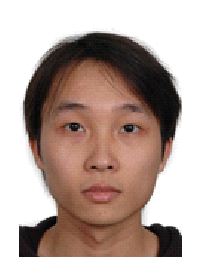
\includegraphics{eps/resume/picture.eps}




\noindent\textbf{教育背景:}\\
(1).~2003年9月$\sim$2007年6月, 中山大学信科院计算机科学与技术专业, 获学士学位。\\
(2).~2007年9月$\sim$2009年6月, 中山大学信科院计算机应用技术专业,硕士研究生。\\

\noindent\textbf{专业经历:} \\
(1).~2007年9月$\sim$至今,中山大学信息与网络中心,研究助理。\\
....................
        %********个人简历
%
\phantomsection

\addcontentsline{toc}{chapter}{\hspace*{0.2cm}致~谢}

\chapter*{ \markboth{致谢}{致谢}}
\vspace{-1cm}\centerline{\xiaoerhao{\hei{致\quad 谢}}}

%\vspace{5mm}{\kai\xiaosihao
论文完成之际,首先感谢中山大学这所高等学府。我在这里学习和生活了六年,这所美丽的学校赋予我许多灵感,也让我有机会结识诸多良师益友。

衷心感谢....

衷心感谢....

衷心感谢....

衷心感谢....

衷心感谢....

最后我要感谢那些在这里不能一一提到的师长、同学和好友,感谢所有帮助和关心过我的人们。谢谢!

%}

%\vspace{2cm}

\hfill {\kai 车春回 \hspace{15mm}

\hfill 2009~年~5~月于康乐园}\hspace{5mm}
        %********致谢
%
\end{document}
